\section{電流・電気抵抗・抵抗の接続と計器}

% ===========================================================================
%  再編（2026-09-24）：第4章 電磁気学 の第26回．
%  原本の 第33回「電流・電気抵抗」の全体（33.1〜33.6）と，
%  第34回「キルヒホッフの法則」の 34.1〜34.3（第一法則／抵抗の直列・並列／電流計・電圧計）を
%  合流させて1回とした．34.4 ホイートストンブリッジの系統的な扱いは第27回へ送る
%  （`saihen/電磁気_例題配分.md` の「第26回で計器まで完結」の通り）．
%
%  ・練習は9題（A問題2題を1題に統合）．練習番号は第25回（［47］〜［59］）の続き．
%      ［60］＝ ㉝[29]＋㉞[36]（A問題の統合。設問は7つとも残した）
%      ［61］＝ ㉝[30]（電流と電荷の移動）      ［62］＝ ㉝[31]（オームの法則・指定）
%      ［63］＝ ㉝[32]（電気抵抗の加速モデル・指定）
%      ［64］＝ ㉝[33]（抵抗の温度変化）        ［65］＝ ㉟[45]（電流計・電圧計）
%      C問題 ［66］＝ ㉝[34]（すべり抵抗）  ［67］＝ ㉝[35]（電池の内部抵抗）
%            ［68］＝ ㉞[41]（合成抵抗・立方体）
%    再編案の「練習10題」は ㉞[36] を独立に数えたもの．A問題2題を統合したので9題になった
%    （設問は1つも失われていない）．
%
%  ・例題は5題．原本の 例題14・15・18・16・19 を講義順に並べた．第25回が【例題6】〜【例題10】
%    なので \setcounter{nombre}{10} として【例題11】〜【例題15】と表示される．
%      【例題11】＝原本14（電流）          【例題12】＝原本15（抵抗モデル）
%      【例題13】＝原本18（合成抵抗）      【例題14】＝原本16（内部抵抗）
%      【例題15】＝原本19（分流器・倍率器）
%
%  ・【重要】原本の講義編（第2冊 20161215144626.pdf）は今回の作業環境に無く，Google Drive からは
%    17MB で取得できなかった（上限10MB）．Drive の OCR テキストだけは取れたので，
%    **例題の問題文はその OCR から復元し，例題の図は circuitikz で描き起こした**
%    （`texify_draft/mkfig_new26ex.py`）．次の点は OCR が崩れていたので推定で補った．要照合：
%      ・例題11(1)「銅$1.00\,\mathrm{cm^3}$中の」（OCR は「中の自由電子は何個か」だけ）．
%        (2) の断面積 $1.00\,\mathrm{mm^2}$（OCR「太さ1.00 [cam?」）．
%      ・例題13 の数値：OCR では抵抗値が読めない（「抵抗/ [0] の3つの」）．指針が
%        「まず$R_2$，$R_3$を合成してから$R_1$を合成する」と文字で書いているので，文字のまま出題した．
%      ・例題14 の点 A〜D の位置：OCR には「内部抵抗$r$，起電力$E$の電池と抵抗$R_1$，$R_2$を
%        直列に接続し，D点を接地した」「A,B,C点の電位を求めよ」しか無い．
%        A＝起電力と内部抵抗の間，B＝電池の正極端子，C＝$R_1$と$R_2$の間 として図を描いた．
%      ・例題15(1) の「$100\U{mA}$まで」（OCR「1000mA)」＝「100[mA]」の括弧の誤読と判断．
%        分流器が$0.20\,\Omega$ちょうどになる）．(5) の「(1)の電流計」は改造前の
%        （内部抵抗$1.8\,\Omega$・最大$10\U{mA}$の）電流計と解釈した．
%    原本には例題の解答が無いので，指針・解答はすべて書き起こした．
%
%  ・原本の本文に無く，練習・例題が前提にしていたものを加筆した（「解答を読んで初めて知る」型の解消）：
%      ・26.1 に「$\overline{v}$は電子の乱雑な運動の速さではない」（原本 p44 の括弧書き＋練習［61］の注）．
%      ・26.6 に「キルヒホッフの第二法則は抵抗を含む回路でもそのまま使える（電圧降下$RI$）」．
%        第二法則は第25回でコンデンサー回路について導入済みなので，その接続だけを書いた．
%      ・26.7 に{端子電圧}$V=E-rI$のまとめ枠．練習［65］［67］の解答がこれを前提にしている．
%      ・26.8 に{分流器・倍率器}の定義（原本では例題19 の指針にしか無かった）．
%      ・26.9 を新設：{等電位の点は導線でつないでも外してもよい}／{対称性で電流分布を決める}／
%        {ブリッジの平衡条件}（練習［60］(7)・［68］が使う．ブリッジの系統的な扱いは第27回）．
%
%  ・原本（問題編の解答）の誤り・不統一を直した（いずれもコメントで明記）：
%      (a) 練習［66］の解答 第1式の左辺「$W=$」→「$E=$」（直後の代入後の式では$E$になっている）．
%      (b) 練習［67］の別解「最大値$\dfrac{V^2}{4R}$」→$\dfrac{V^2}{4r}$（$R=r$を代入した値なので
%          どちらでも同じ値だが，最大値は$r$で書くべき）．
%      (c) 単位を \U{} に，強調を {\gtfamily } に統一．wrapfigure は使わず zuright / center だけで組んだ．
%
%  ・図：講義の図は講義編から切り出し済みのもの（img/text/text2_p44〜p55）をそのまま使う．
%    練習・解答の図は `texify_draft/mkfig_new26.py`＋`jobs_new26.py`，例題の図は `mkfig_new26ex.py`．
% ===========================================================================

% 例題番号：第25回が【例題6】〜【例題10】
\setcounter{nombre}{10}

\subsection{電流}

\begin{zuright}{40mm}
\hspace{1zw}コンデンサー回路で見られたような，電荷が移動する現象のことを{\gtfamily 電流}と呼ぶ．
電流の大きさは，導線のある点（断面）を{\gtfamily 単位時間あたりに通過する電気量}として定義されている．
すなわち，図の点$\mathrm{a}$を微小時間$dt\U{s}$の間に微小電荷$dQ\U{C}$が通過するとき，この点を流れる電流を，図の矢印の向きに
\zusep

\includegraphics[keepaspectratio,width=40mm]{text2_p44_fig1.png}
\end{zuright}
\AnaBD{I=\frac{dQ}{dt}\U{A}}
として定義する．
電流の単位は$\U{A}$（アンペア）であるが，この定義より$\U{A}=\U{C/s}$である．

電流の向きは回路中を{\gtfamily 正電荷が動いていく向き}として決められているが，実際に導線中を動いていくのは電子である．
電子の持つ電荷は$-e\U{C}$，すなわち負であるから，電流が図の向きに流れているということは，{\gtfamily 電子がそれと逆向きに動いている}ということを意味する．

\begin{zuright}{70mm}
\hspace{1zw}導体中（金属中）では，金属結晶を構成する陽イオンの間を自由電子が自由に動き回っているが，これに図のように電池を接続して電場を生じさせると，電子は陽イオンに衝突しながらも全体として高電位側へと移動していく．

\hspace{1zw}導体中の自由電子の単位体積あたりの個数を$n\U{/m^3}$，導線の断面積を$S\U{m^2}$，自由電子の平均移動速度を$\overline{v}\U{m/s}$とする．
時間$\varDelta t$の間にある断面を通過するのは，その断面から長さ$\overline{v}\varDelta t$の範囲にある$n\cdot S\overline{v}\varDelta t$個の電子であるから，通過する電気量は$e\cdot nS\overline{v}\varDelta t$である．
\zusep

\includegraphics[keepaspectratio,width=70mm]{text2_p44_fig2.png}
\end{zuright}
これを$\varDelta t$で割れば，流れる電流$I\U{A}$は
\AnaBD{I=en\overline{v}S\U{A}}
で与えられる．
% 加筆：原本 p44 の括弧書き「自由電子の平均の速さとは異なることに注意」を本文に出した（練習［61］の注が前提にしている）．
ここで$\overline{v}$は電子の集団が全体として流れていく速さ（{\gtfamily 平均移動速度}）であって，電子1個1個が陽イオンの間を乱雑に飛び回る速さ（熱運動の速さ）とは{\gtfamily まったく別のもの}である．
例題11で見るように，$\overline{v}$は$10^{-4}\U{m/s}$程度と非常に遅い．

\bsNeed{26mm}
\begin{matome}{電流}
 \hspace{3mm} 電流の定義\quad $I=\dfrac{dQ}{dt}\U{A}$ \hspace{12mm} 導線を流れる電流\quad $I=en\overline{v}S\U{A}$
\end{matome}

%%%%%%%%%%  例題11（原本の【例題14】）  %%%%%%%%%%%%%%%%%%%%
\bsNeed{70mm}
\begin{reidaiunit}
\begin{reidai}{電流}
\hspace{1zw}銅（原子量$63.5$，密度$8.93\U{g/cm^3}$）は1原子あたり1個の自由電子を放出する．電子の電荷を$-e=-1.60\times 10^{-19}\U{C}$，アボガドロ定数を$N_{\mathrm{A}}=6.02\times 10^{23}\U{/mol}$として，以下の設問に答えよ．
\begin{komon}
\ko{1} 銅$1.00\U{cm^3}$中の自由電子は何個か．
\ko{2} 断面積$1.00\U{mm^2}$の銅線に$2.00\U{A}$の電流が流れているとき，自由電子の平均移動速度$\overline{v}\U{m/s}$を求めよ．
\end{komon}
\end{reidai}

\begin{sisinE}
(1) 原子量$63.5$とは，1\,molあたりの質量が$63.5\U{g}$ということである．$1.00\U{cm^3}$の質量を密度から出し，それが何molかを考えれば原子の数，すなわち自由電子の数が分かる．

(2) $I=en\overline{v}S$を$\overline{v}$について解くだけであるが，{\gtfamily 単位をすべて$\U{m}$系に直してから代入する}こと．$n$は$1\U{m^3}$あたりの個数であり，$1\U{cm^3}=10^{-6}\U{m^3}$，$1\U{mm^2}=10^{-6}\U{m^2}$である．
\end{sisinE}

\Key{$I=en\overline{v}S\U{A}$（$n$：単位体積あたりの自由電子数，$\overline{v}$：平均移動速度）}

\begin{kaitou}
\begin{komon}
\ko{1} $1.00\U{cm^3}$の銅の質量は$8.93\U{g}$であり，物質量は$\dfrac{8.93}{63.5}\U{mol}$である．1原子あたり1個の自由電子を出すので，
       \[N=\frac{8.93}{63.5}\times 6.02\times 10^{23}\fallingdotseq 8.47\times 10^{22}\ \text{個}\Ans\]
\ko{2} (1)より，$1\U{m^3}$あたりの自由電子数は$n=8.47\times 10^{22}\times 10^{6}=8.47\times 10^{28}\U{/m^3}$である．$S=1.00\times 10^{-6}\U{m^2}$として$I=en\overline{v}S$より
       \Ana{\overline{v}=\frac{I}{enS}=\frac{2.00}{1.60\times 10^{-19}\times 8.47\times 10^{28}\times 1.00\times 10^{-6}}\fallingdotseq 1.48\times 10^{-4}\U{m/s}\Ans}
       \begin{chuu}
       $1.5\times 10^{-4}\U{m/s}$は1秒間に$0.15\U{mm}$しか進まない速さである．それでもスイッチを入れると電灯がすぐにつくのは，電場が導線全体にほぼ一瞬で伝わり，{\gtfamily 導線中のすべての自由電子が一斉に動き出す}からである．
       \end{chuu}
\end{komon}
\end{kaitou}
\end{reidaiunit}

\subsection{オームの法則とジュール熱}

導線の両端に電圧をかけると，これにより電場が生じて電流が流れるが，一般に，流れる電流$I\U{A}$とかける電圧$V\U{V}$との間には比例関係が成り立つ．
\AnaBD{V=RI}
これを{\gtfamily オームの法則}といい，比例定数$R$を{\gtfamily 抵抗値（電気抵抗）}と呼ぶ．
抵抗値の単位は上式より$\U{V/A}$であるが，これを$\U{\Omega}$（オーム）と書く．
抵抗値は{\gtfamily 電流の流れにくさ}を表す量であり，その材質，長さ，太さ，温度により決まる．

電気抵抗が非常に大きな物質を{\gtfamily 絶縁体（誘電体）}，中程度のものを{\gtfamily 半導体}，小さいものを{\gtfamily 導体}と呼ぶ．
回路の問題では，特に断りがなければ{\gtfamily 導線（金属）の抵抗は$0\U{\Omega}$}として扱ってよい．

\begin{zuright}{56mm}
\hspace{1zw}例えば図のように，抵抗値$R\U{\Omega}$の抵抗を電流$I\U{A}$が流れるとき，抵抗内の電位は電流が流れる向きに一様に下がっていき，抵抗の前後では$RI\U{V}$だけ電位が変化している．
すなわち，{\gtfamily 電流の流れる向きに沿って，抵抗の前後で電位が$RI$だけ下がる}．
この電位の変化を抵抗による{\gtfamily 電圧降下}という．
電気抵抗を組み合わせて作られる回路は，この電圧降下とキルヒホッフの法則（26.6）を組み合わせて考えていく．

\hspace{1zw}電流が流れている抵抗からは{\gtfamily ジュール熱}と呼ばれる熱が発生する．
その熱量は，$1\U{s}$あたり
\[P=VI=RI^2=\frac{V^2}{R}\U{J/s}\]
である．これを抵抗で消費される{\gtfamily 電力}という．単位$\U{J/s}$を$\U{W}$（ワット）と書く．
\zusep

\includegraphics[keepaspectratio,width=56mm]{text2_p45_fig1.png}
\end{zuright}

電荷$q$が電位差$V$だけ低いところへ移ると，電場は$qV$の仕事をする．
抵抗の中では$1\U{s}$あたり$I\U{C}$の電荷が$V$だけ電位を下げるので，電場は毎秒$VI$の仕事をしており，これが陽イオンとの衝突を通じて熱に変わる（例題12・練習［63］で詳しく見る）．

また，電気抵抗$R\U{\Omega}$は導線の長さ$l\U{m}$に比例し，断面積$S\U{m^2}$に反比例することが知られている．
比例定数を$\rho\U{\Omega\cdot m}$として
\AnaBD{R=\rho\frac{l}{S}\U{\Omega}}
と書くことができる．$\rho$は導線の材質（と温度）によって決まる定数で，これを{\gtfamily 抵抗率}とよぶ．
長い導線ほど電流が流れにくく，太い導線ほど流れやすい，と考えれば分母・分子を取り違えない．

\bsNeed{26mm}
\begin{matome}{電気抵抗}
 \hspace{3mm} $V=RI\U{V}$ \hspace{10mm} $P=VI=RI^2=\dfrac{V^2}{R}\U{W}$ \hspace{10mm} $R=\rho\dfrac{l}{S}\U{\Omega}$
\end{matome}

\subsection{電気抵抗のモデル}

そもそも電気抵抗は，自由電子が動こうとする際に導体中の陽イオンに衝突するため，スムーズに進めないことが原因となって生じる．
よって原理的には，導体中の電子の運動を考えれば電気抵抗が生じる理由を説明できるはずである．

しかし，導体中の電子の運動を運動方程式に従って厳密に記述し，それを解くのは数学的にも容易ではない．
そこで，現象をある程度単純化してとらえ，およそどのような振る舞いをするのかを考える．
これを現象の{\gtfamily モデル化}という．
電気抵抗の場合，次の例題のような「抵抗力モデル」を考えると，オームの法則や抵抗率の式を説明することができる（別のモデル「加速モデル」を練習［63］で扱う）．

%%%%%%%%%%  例題12（原本の【例題15】）  %%%%%%%%%%%%%%%%%%%%
\bsNeed{120mm}
\begin{reidaiunit}
\begin{reidai}{抵抗モデルによる電気抵抗の記述}
\begin{zuright}{58mm}
\hspace{1zw}金属導体中の自由電子は，金属結晶を構成する陽イオンと衝突を繰り返しながら導体内で熱運動をしているが，この導線に電圧をかけると導線内に電場が生じ，自由電子は陽イオンと衝突しながらも全体としては電場とは逆向きに一定の速さ$v\U{m/s}$（平均移動速度）で動いていき，これが電流となる．
電子の電荷を$-e\U{C}$とし，単位体積中の自由電子の個数を$n\U{/m^3}$，断面積$S\U{m^2}$，長さ$l\U{m}$の導線に電圧$V\U{V}$をかける場合に流れる電流について以下の問いに答えよ．
\zusep
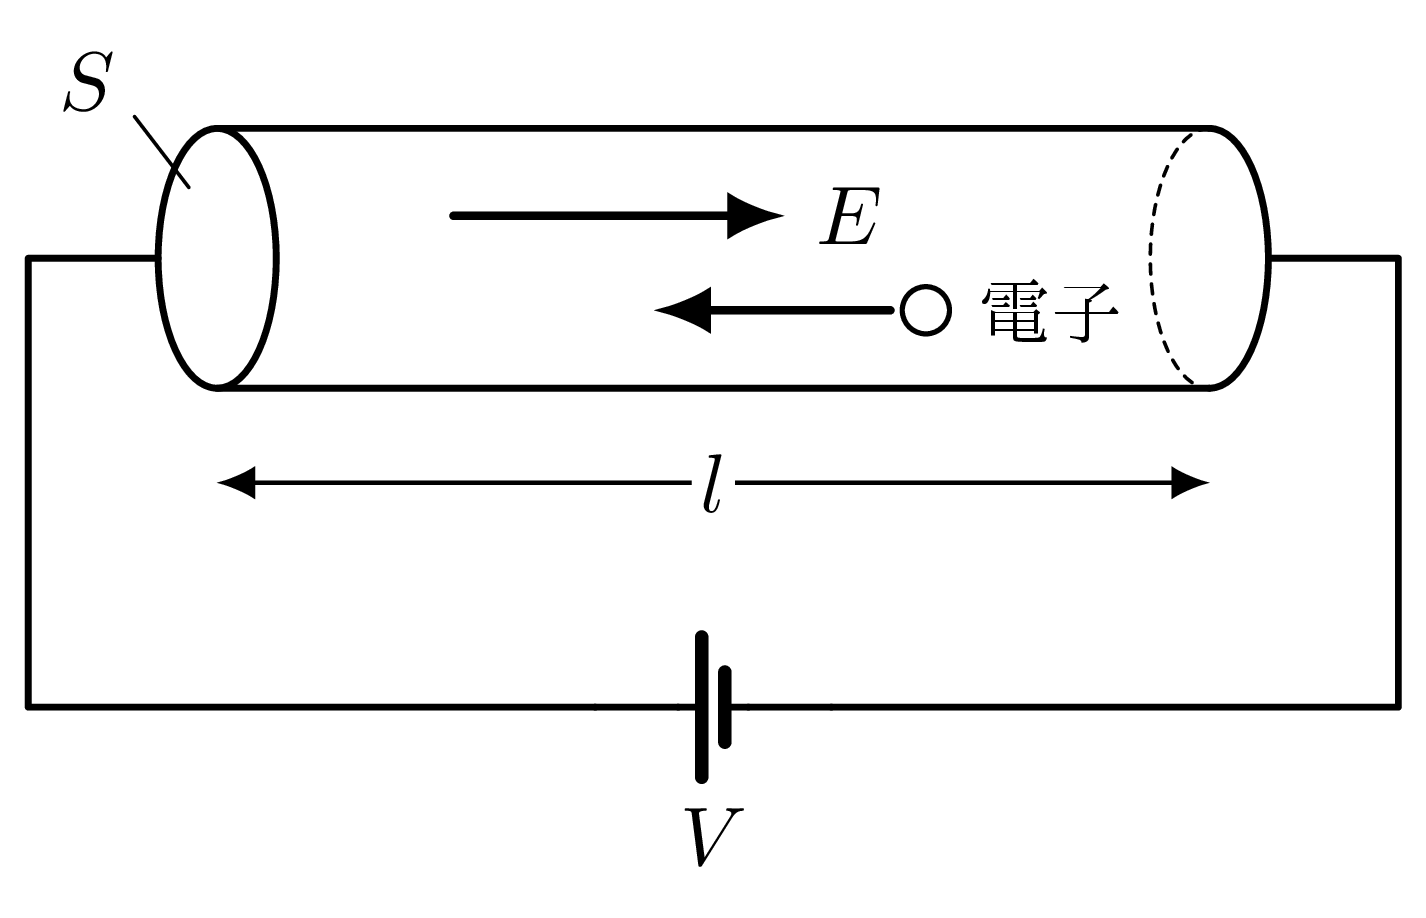
\includegraphics[keepaspectratio,width=58mm]{fig/n26_ex12_zu.png}
\end{zuright}
\begin{komon}
\ko{1} 導線に流れる電流$I\U{A}$を表せ．
\ko{2} 電圧$V\U{V}$をかけたことにより導線内に生じる電場の大きさ$E\U{N/C}$を求めよ．
\end{komon}
\hspace{1zw}この電場により電子は導線内を電場と逆向きに移動していくが，電子は陽イオンとの衝突により，電場から受ける力とは逆向きにはね返されたりする．このことを，電子が平均移動速度の向きとは逆向きに陽イオンから抵抗力を受けることだと解釈する．反発は電子の移動する速さが大きいほど強いと考えられるので，受ける抵抗力の大きさを$kv\U{N}$（ただし$k\U{N\cdot s/m}$は定数）であるとする．
\begin{komon}
\ko{3} 定常状態では電子は平均して一定の速さで導線中を移動していく．このことから，導線中を移動する電子の平均移動速度$v\U{m/s}$を求めよ．
\ko{4} この導線の抵抗$R\U{\Omega}$および抵抗率$\rho\U{\Omega\cdot m}$を求めよ．
\ko{5} 電場$E\U{N/C}$が1つの電子に対して単位時間あたりにしている仕事（仕事率）を求めよ．
\ko{6} 電場は電子に対して仕事をしているが，定常状態においては電子の速さ$v\U{m/s}$は不変である．これは電子が陽イオンと衝突することにより陽イオンに熱エネルギーを与えているからである．このことから，1つの電子が単位時間あたりに陽イオンに与えるエネルギーを求めよ．
\ko{7} 導線全体で単位時間あたりに発生する熱エネルギーを$k$，$e$，$n$，$S$，$l$，$V$で表し，さらに$R$，$V$でまとめよ．
\end{komon}
\end{reidai}

\begin{sisinE}
生じる電場の向き，電子が受ける力の向きに注意して考えていくこと．
電子の電荷は負なので，電子は電場と逆向きに$eE$の力を受ける．
定常状態では電子の速さが一定なので，{\gtfamily 電場からの力$eE$と抵抗力$kv$がつり合っている}．
これが(3)の立式であり，この「つり合いの速さ」が電流の大きさを決める．

(5)〜(7)はエネルギーの見方である．力$F$の向きに速さ$v$で動く物体に対して，力は単位時間あたり$Fv$の仕事をする．
\end{sisinE}

\Key{$I=envS$\quad 一様な電場$E=\dfrac{V}{l}$\quad 定常状態では力がつり合う\quad 仕事率$=Fv$}

\begin{kaitou}
\begin{komon}
\ko{1} 26.1 と同様に，
       \[I=envS\U{A}\Ans\]
\ko{2} 長さ$l$の導線の両端に電位差$V$がかかり，導線内には一様な電場ができるので，
       \[E=\frac{V}{l}\U{N/C}\Ans\]
\ko{3} 1個の電子には，電場から$eE$の力（電場と逆向き），陽イオンから$kv$の抵抗力（運動と逆向き）がはたらく．定常状態では速さが一定なので，この2力がつり合う：
       \Ana{eE=kv\qquad\therefore\ v=\frac{eE}{k}=\frac{eV}{kl}\U{m/s}\Ans}
\ko{4} (1)に(3)を代入して
       \[I=en\cdot\frac{eV}{kl}\cdot S=\frac{e^2nS}{kl}V\]
       これが$V=RI$の形になっているので
       \[R=\frac{kl}{e^2nS}\U{\Omega}\Ans\]
       $R=\rho\dfrac{l}{S}$と比べて
       \[\rho=\frac{k}{e^2n}\U{\Omega\cdot m}\Ans\]
       \begin{chuu}
       電流が電圧に比例する（オームの法則）こと，抵抗が$l$に比例し$S$に反比例することが，このモデルから導かれた．$\rho$は$k$と$n$，すなわち材質だけで決まり，形によらない．
       \end{chuu}
\ko{5} 電子は電場からの力$eE$の向きに速さ$v$で動いているので，単位時間あたりの仕事は
       \[eE\cdot v=\frac{eV}{l}\cdot\frac{eV}{kl}=\frac{e^2V^2}{kl^2}\U{W}\Ans\]
\ko{6} 速さが変わらないので，電場からもらったエネルギーはすべて衝突で陽イオンに渡される．よって(5)と同じく
       \[\frac{e^2V^2}{kl^2}\U{W}\Ans\]
       （抵抗力$kv$が単位時間にする負の仕事$kv\cdot v$を計算しても同じ値になる）
\ko{7} 導線内の自由電子の総数は$nSl$個なので，
       \[P=\frac{e^2V^2}{kl^2}\times nSl=\frac{e^2nS}{kl}V^2\U{W}\Ans\]
       (4)の$R=\dfrac{kl}{e^2nS}$を用いれば
       \[P=\frac{V^2}{R}\U{W}\Ans\]
       となり，26.2 のジュール熱の式と一致する．
\end{komon}
\end{kaitou}
\end{reidaiunit}

\subsection{抵抗の温度係数}

\begin{zuright}{62mm}
\hspace{1zw}抵抗値$R\U{\Omega}$および抵抗率$\rho\U{\Omega\cdot m}$の値は一定ではなく，温度によって変化する．
例えば金属の場合，電子は図のように陽イオンと衝突を繰り返しつつ移動していくが，温度が高くなると陽イオンの熱振動が大きくなり，電子との衝突が起こりやすくなるので抵抗値が大きくなる．
\zusep

\includegraphics[keepaspectratio,width=62mm]{text2_p47_fig1.png}
\end{zuright}
温度$0\U{^\circ C}$における抵抗値，抵抗率をそれぞれ$R_0\U{\Omega}$，$\rho_0\U{\Omega\cdot m}$，温度$t\U{^\circ C}$における抵抗値，抵抗率をそれぞれ$R\U{\Omega}$，$\rho\U{\Omega\cdot m}$とすると，よい近似で
\[R=R_0(1+\alpha t)\U{\Omega}\qquad \rho=\rho_0(1+\alpha t)\U{\Omega\cdot m}\]
が成り立つ．$\alpha\U{/K}$を抵抗値（抵抗率）の{\gtfamily 温度係数}という．
温度係数は{\gtfamily 金属では正の値，半導体（ケイ素，ゲルマニウムなど）では負の値}となる．

\begin{zuright}{40mm}
\hspace{1zw}金属の抵抗にかける電圧を高くするとジュール熱が多くなり，抵抗の温度が上がるため電流はより流れにくくなる．
そのため，通常の金属の抵抗ではオームの法則は厳密には成立せず，$I$-$V$特性曲線は図の実線のように原点を通る直線（点線）より下に曲がっていく．
オームの法則が完全に成立する理想的な抵抗のことを{\gtfamily オーム抵抗}と呼び，図のようなオームの法則に従わない抵抗を{\gtfamily 非オーム抵抗}と呼ぶ．
通常，断りのない限り抵抗はオーム抵抗として扱ってよい（非オーム抵抗を含む回路は第27回で扱う）．
\zusep

\includegraphics[keepaspectratio,width=40mm]{text2_p47_fig2.png}
\end{zuright}

\bsNeed{30mm}
\begin{matome}{抵抗値・抵抗率の温度依存性}
 \[R=R_0(1+\alpha t)\U{\Omega}\hspace{10mm}\rho=\rho_0(1+\alpha t)\U{\Omega\cdot m}\]
 \hspace{3mm} $R_0$，$\rho_0$は温度$0\U{^\circ C}$における値．温度係数$\alpha\U{/K}$は\,\AnaB{金属では正}，\AnaB{半導体では負}
\end{matome}

\subsection{半導体}

\begin{zuright}{56mm}
\hspace{1zw}14族の元素$\mathrm{Si}$や$\mathrm{Ge}$の結晶は共有結合による結合からなる．
実際には3次元的に結合しているが，図では便宜上2次元的に表している．

\hspace{1zw}十分に低温であれば，価電子はすべて共有結合に使われていて，自由に動ける荷電粒子（電荷の担い手）が結晶内にないので，電流は流れない．

\hspace{1zw}しかし，温度が高くなると電子は大きなエネルギーを持つようになり，この束縛を振り切って自由になる電子ができる．
このように自由電子ができると，その電子が抜けたあとに電子の穴ができる．この穴を{\gtfamily 正孔（ホール）}という．
\zusep

\includegraphics[keepaspectratio,width=56mm]{text2_p48_fig1.png}
\end{zuright}
こうしてできた自由電子は，金属中の自由電子と同じように電流の担い手（これを{\gtfamily キャリア}と呼ぶ）となり得る．
正孔も，周りにある電子がこの穴に落ち込むことによって位置を変えることができるので，自由電子と同様に半導体内を動けるキャリアとなる．
このように，{\gtfamily 自由電子は負の電荷を運ぶキャリア，正孔は正の電荷を運ぶキャリア}と考えてよい．

\begin{center}

\includegraphics[keepaspectratio,width=130mm]{text2_p48_fig2.png}
\end{center}

温度が高いほど，半導体内にある自由電子と正孔の数は増える．
その結果，{\gtfamily 半導体では温度が高いほど抵抗値が小さくなる}ことが多い．
金属の場合は温度が上がっても電子の密度はほとんど変わらず，格子の振動によって抵抗値が増加する．
もちろん半導体でも格子振動の影響はあるので，温度上昇に伴って抵抗値が必ず下がるとは限らない．

\begin{zuright}{40mm}
\hspace{1zw}純粋な半導体は常温では電子，正孔ともにあまり発生しないが，不純物を少し混ぜることによってキャリアが発生しやすくなる．
このような半導体を{\gtfamily 不純物半導体}といい，混入する不純物の種類によって$\mathrm{N}$型半導体，$\mathrm{P}$型半導体に分けられる．

\hspace{1zw}15族の元素（例えば$\mathrm{P}$や$\mathrm{As}$）を混入すると，共有結合の際に電子が1つ余る．
この余った電子は不純物の周りに電気的に引きつけられているが，その束縛は弱く，容易に自由電子となる．
\zusep

\includegraphics[keepaspectratio,width=40mm]{text2_p48_fig3.png}
\end{zuright}
このような半導体を{\gtfamily $\mathrm{N}$型半導体}（$\mathrm{N}$は negative の$\mathrm{N}$）といい，不純物を{\gtfamily ドナー}と呼ぶ．
$\mathrm{N}$型半導体のキャリアは主に電子である．

一方，13族の元素（例えば$\mathrm{Al}$や$\mathrm{Ga}$）を混入すると，共有結合の電子が1つ足りなくなるので，負に帯電した不純物の周りに正孔が束縛され，自由に動ける正孔ができやすい．
このような半導体を{\gtfamily $\mathrm{P}$型半導体}（$\mathrm{P}$は positive の$\mathrm{P}$）といい，不純物を{\gtfamily アクセプター}と呼ぶ．
$\mathrm{P}$型半導体のキャリアは主に正孔である．
$\mathrm{P}$型と$\mathrm{N}$型をつないだダイオードは第27回で扱う．

\begin{center}

\includegraphics[keepaspectratio,width=120mm]{text2_p49_fig1.png}
\end{center}

\subsection{キルヒホッフの第一法則と抵抗の接続}

\begin{zuright}{58mm}
\hspace{1zw}ここまでは回路に枝分かれのないものを扱ってきたが，枝分かれのある回路を扱うときには次の{\gtfamily キルヒホッフの第一法則}を考える必要がある．
電流は電荷の流れであり，電荷はコンデンサーの極板上以外には長時間とどまることができない．
そのため，{\gtfamily 回路の分岐点に流れ込む電流の和と，その点から流れ出ていく電流の和とは必ず等しくなる}．
これをキルヒホッフの第一法則という（電荷保存の法則の言い換えである）．
\zusep

\includegraphics[keepaspectratio,width=58mm]{text2_p51_fig1.png}
\end{zuright}

% 加筆：第二法則はコンデンサー回路（第25回 25.4）で導入済み．抵抗を含む場合の立式の形をここで接続する．
一方，{\gtfamily キルヒホッフの第二法則}（回路の閉ループをひと回りすると電位はもとに戻る）はコンデンサー回路（25.4）で学んだが，抵抗を含む回路でもそのまま成り立つ．
抵抗では電流の向きに$RI$だけ電位が下がるので，閉ループに沿って
\[\sum(\text{起電力})=\sum(\text{電圧降下 }RI)\]
と立式すればよい．
この2つの法則を併用すれば，抵抗と電池からなる回路に流れる電流を計算することができる．
各導線の電流を未知数として置いていくとき，{\gtfamily 先に第一法則で未知数を減らしておく}と楽になることが多い．

\bsNeed{34mm}
\begin{matome}{キルヒホッフの法則}
 {\gtfamily 第一法則}\quad 回路の分岐点に流れ込む電流の和と流れ出ていく電流の和とは等しい\\
 {\gtfamily 第二法則}\quad 任意の閉ループで\ \AnaB{起電力の代数和＝電圧降下の代数和}
\end{matome}

複数の抵抗をつないだものを，あたかも1つの抵抗であるかのように扱うことができる．
これを{\gtfamily 抵抗の合成}といい，うまく用いると連立方程式を立てずに流れる電流を計算できる．

\bsNeed{56mm}
\begin{zuright}{50mm}
\noindent\MARU{1}\ {\gtfamily 直列接続 $\cdots$ すべての抵抗に同じ電流が流れる}

\hspace{1zw}$R_1$，$R_2$，$R_3\U{\Omega}$の3つの抵抗を図のように直列に接続し，電流$I\U{A}$を流すと，各抵抗の電圧降下は$R_1I$，$R_2I$，$R_3I\U{V}$であり，$\mathrm{ab}$間の電位差は
\[V_{\mathrm{ab}}=(R_1+R_2+R_3)I\U{V}\]
である．これを$V_{\mathrm{ab}}=RI$と書けば，合成抵抗は
\[R=R_1+R_2+R_3\U{\Omega}\]
である．各抵抗の電圧の比は$R_1:R_2:R_3$（抵抗値の比）となる．
\zusep

\includegraphics[keepaspectratio,width=50mm]{text2_p52_fig1.png}
\end{zuright}

\bsNeed{60mm}
\begin{zuright}{46mm}
\noindent\MARU{2}\ {\gtfamily 並列接続 $\cdots$ すべての抵抗に同じ電圧がかかる}

\hspace{1zw}$R_1$，$R_2$，$R_3\U{\Omega}$の3つの抵抗を図のように並列に接続し，$\mathrm{ab}$間に電圧$V_{\mathrm{ab}}\U{V}$をかけると，各抵抗には$\dfrac{V_{\mathrm{ab}}}{R_1}$，$\dfrac{V_{\mathrm{ab}}}{R_2}$，$\dfrac{V_{\mathrm{ab}}}{R_3}\U{A}$の電流が流れる．
キルヒホッフの第一法則より，端子$\mathrm{a}$に流れ込む電流$I\U{A}$は
\[I=\Bigl(\frac{1}{R_1}+\frac{1}{R_2}+\frac{1}{R_3}\Bigr)V_{\mathrm{ab}}\U{A}\]
である．これを$I=\dfrac{V_{\mathrm{ab}}}{R}$と書けば，合成抵抗は
\[\frac{1}{R}=\frac{1}{R_1}+\frac{1}{R_2}+\frac{1}{R_3}\]
を満たす．各抵抗の電流の比は$\dfrac{1}{R_1}:\dfrac{1}{R_2}:\dfrac{1}{R_3}$（抵抗値の逆数の比）となる．
\zusep

\includegraphics[keepaspectratio,width=46mm]{text2_p52_fig2.png}
\end{zuright}

\bsNeed{30mm}
\begin{matome}{合成抵抗}
 \hspace{3mm} {\gtfamily 直列}接続：合成抵抗は各抵抗値の{\gtfamily 和}\hspace{24mm}\AnaBD{R=R_1+R_2+R_3}\\
 \hspace{3mm} {\gtfamily 並列}接続：合成抵抗の{\gtfamily 逆数}は各抵抗値の{\gtfamily 逆数の和}\hspace{5mm}\AnaBD{\frac{1}{R}=\frac{1}{R_1}+\frac{1}{R_2}+\frac{1}{R_3}}
\end{matome}

%%%%%%%%%%  例題13（原本の【例題18】）  %%%%%%%%%%%%%%%%%%%%
\bsNeed{70mm}
\begin{reidaiunit}
\begin{reidai}{合成抵抗}
\begin{zuright}{56mm}
\hspace{1zw}抵抗値$R_1$，$R_2$，$R_3\U{\Omega}$の3つの抵抗と，内部抵抗の無視できる起電力$E\U{V}$の電池を図のように接続した．このとき，以下の設問に答えよ．
\begin{komon}
\ko{1} $\mathrm{ab}$2点間の合成抵抗の値を求めよ．
\ko{2} 各抵抗に流れる電流の大きさをそれぞれ求めよ．
\end{komon}
\zusep
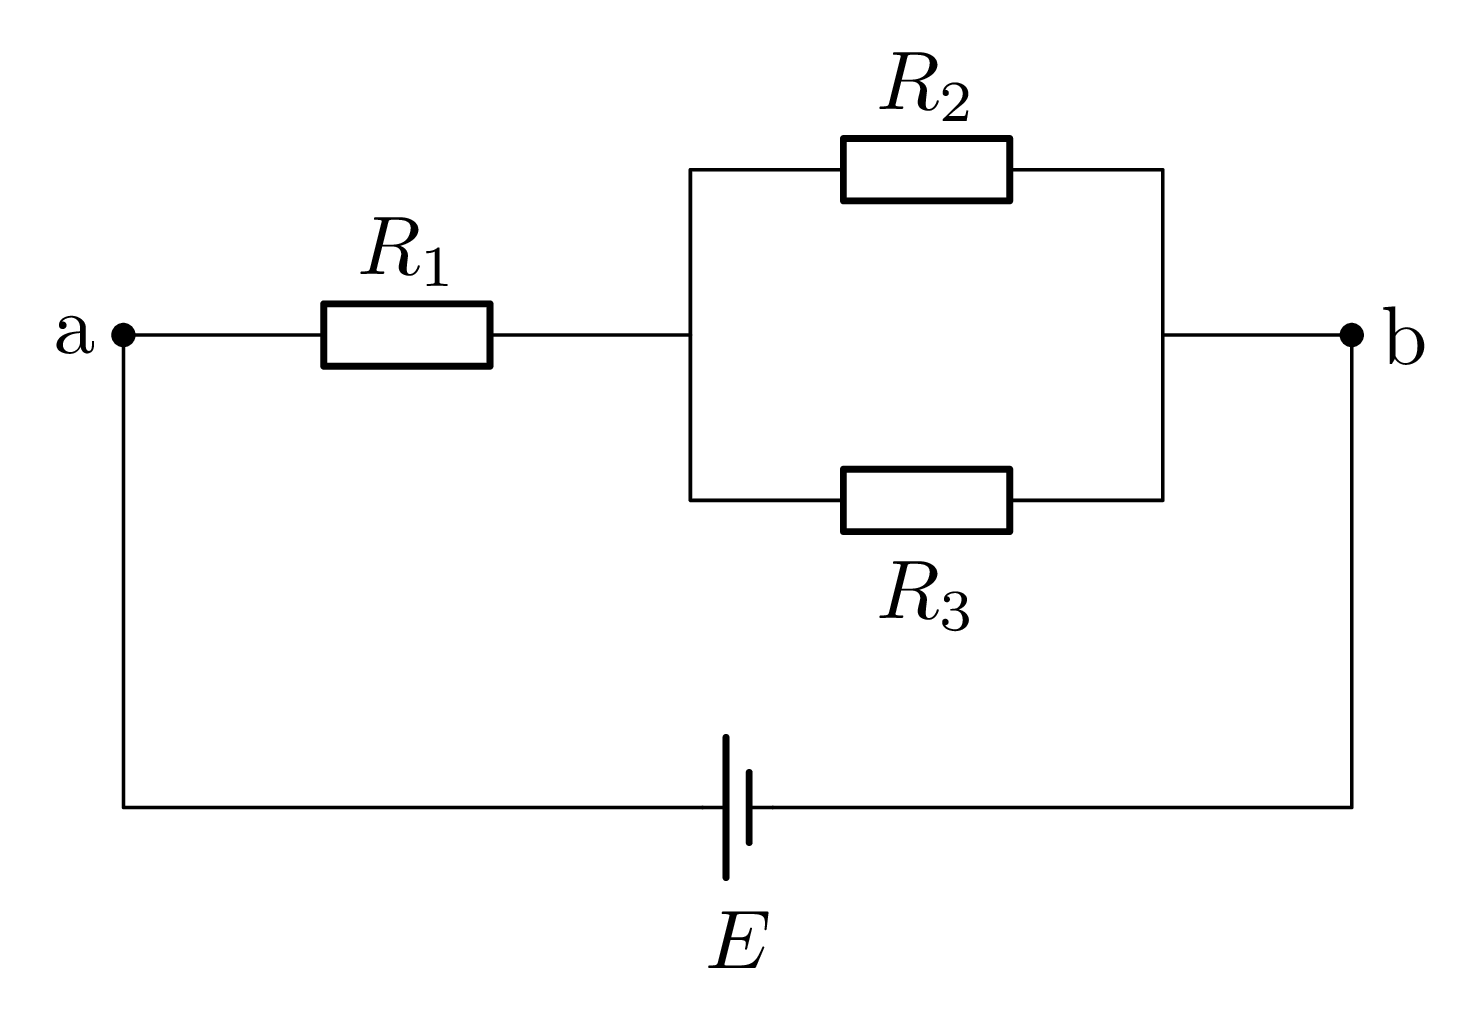
\includegraphics[keepaspectratio,width=56mm]{fig/n26_ex13_zu.png}
\end{zuright}
\end{reidai}

\begin{sisinE}
(1) まず並列部分の$R_2$，$R_3$を合成してから，それと直列の$R_1$を合成する．

(2) 合成抵抗から求められる電流は$\mathrm{a}$，$\mathrm{b}$点を通過する電流，すなわち$R_1$を流れる電流である．
その電流が$R_2$と$R_3$にどう分配されるかを考える．並列部分には共通の電圧がかかるので，まずその電圧を求めるとよい．
\end{sisinE}

\Key{直列：$R=R_1+R_2$\quad 並列：$\dfrac{1}{R}=\dfrac{1}{R_1}+\dfrac{1}{R_2}$\quad 並列部分には同じ電圧がかかる}

\begin{kaitou}
\begin{komon}
\ko{1} $R_2$と$R_3$の並列部分の合成抵抗は
       \[\Bigl(\frac{1}{R_2}+\frac{1}{R_3}\Bigr)^{-1}=\frac{R_2R_3}{R_2+R_3}\]
       であり，これと$R_1$が直列なので
       \Ana{R=R_1+\frac{R_2R_3}{R_2+R_3}=\frac{R_1R_2+R_2R_3+R_3R_1}{R_2+R_3}\U{\Omega}\Ans}
\ko{2} $R_1$を流れる電流（$\mathrm{a}$，$\mathrm{b}$を通過する電流）は
       \[I_1=\frac{E}{R}=\frac{(R_2+R_3)E}{R_1R_2+R_2R_3+R_3R_1}\U{A}\Ans\]
       並列部分にかかる電圧は
       \[V=\frac{R_2R_3}{R_2+R_3}I_1=\frac{R_2R_3E}{R_1R_2+R_2R_3+R_3R_1}\]
       であるから，
       \[I_2=\frac{V}{R_2}=\frac{R_3E}{R_1R_2+R_2R_3+R_3R_1}\U{A}\Ans\]
       \[I_3=\frac{V}{R_3}=\frac{R_2E}{R_1R_2+R_2R_3+R_3R_1}\U{A}\Ans\]
       \begin{chuu}
       $I_2+I_3=I_1$（キルヒホッフの第一法則）になっていること，$I_2:I_3=R_3:R_2$（抵抗値の逆数の比）になっていることを確かめておくとよい．
       \end{chuu}
\end{komon}
\end{kaitou}
\end{reidaiunit}

\subsection{電池の内部抵抗}

\begin{zuright}{34mm}
\hspace{1zw}電池は金属のイオン化傾向の違いなどを利用して電圧を発生させるものであるが，内部に電解質溶液などを用いているため，電池自身もごくわずかではあるが抵抗を持つ．
これを電池の{\gtfamily 内部抵抗}という．
そのため，電池が電流を流し出すとその端子間の電圧は小さくなる．
電流を流していない状態における電池の端子間の電圧を，その電池の{\gtfamily 起電力}と呼ぶ．
\zusep

\includegraphics[keepaspectratio,width=34mm]{text2_p50_fig1.png}
\end{zuright}

内部抵抗は一般には小さいため無視してよいことが多いが，無視できない場合には{\gtfamily 電池を「起電力だけを持つ理想的な電池」と「内部抵抗」の直列に書き直して考える}．

% 加筆：端子電圧の式．練習［65］［67］の解答が前提にしている．
起電力$E\U{V}$，内部抵抗$r\U{\Omega}$の電池が電流$I\U{A}$を流し出しているとき，内部抵抗で$rI$の電圧降下があるので，電池の端子間の電圧（{\gtfamily 端子電圧}）は
\[V=E-rI\U{V}\]
となる．流す電流が大きいほど端子電圧は下がる．

\bsNeed{26mm}
\begin{matome}{内部抵抗のある電池}
 \hspace{3mm} 起電力$E$と内部抵抗$r$の直列に書き直す\hspace{12mm}端子電圧\quad\AnaBD{V=E-rI\U{V}}
\end{matome}

%%%%%%%%%%  例題14（原本の【例題16】）  %%%%%%%%%%%%%%%%%%%%
\bsNeed{76mm}
\begin{reidaiunit}
\begin{reidai}{内部抵抗}
\begin{zuright}{58mm}
\hspace{1zw}内部抵抗$r\U{\Omega}$，起電力$E\U{V}$の電池と，抵抗値$R_1$，$R_2\U{\Omega}$の抵抗を図のように直列に接続し，$\mathrm{D}$点を接地した．点$\mathrm{A}$は電池の内部で起電力と内部抵抗の間にある点，点$\mathrm{B}$は電池の正極の端子である．これについて以下の設問に答えよ．
\begin{komon}
\ko{1} このとき回路を流れる電流の大きさを求めよ．
\ko{2} この状態における$\mathrm{A}$，$\mathrm{B}$，$\mathrm{C}$点の電位を求めよ．
\end{komon}
\zusep
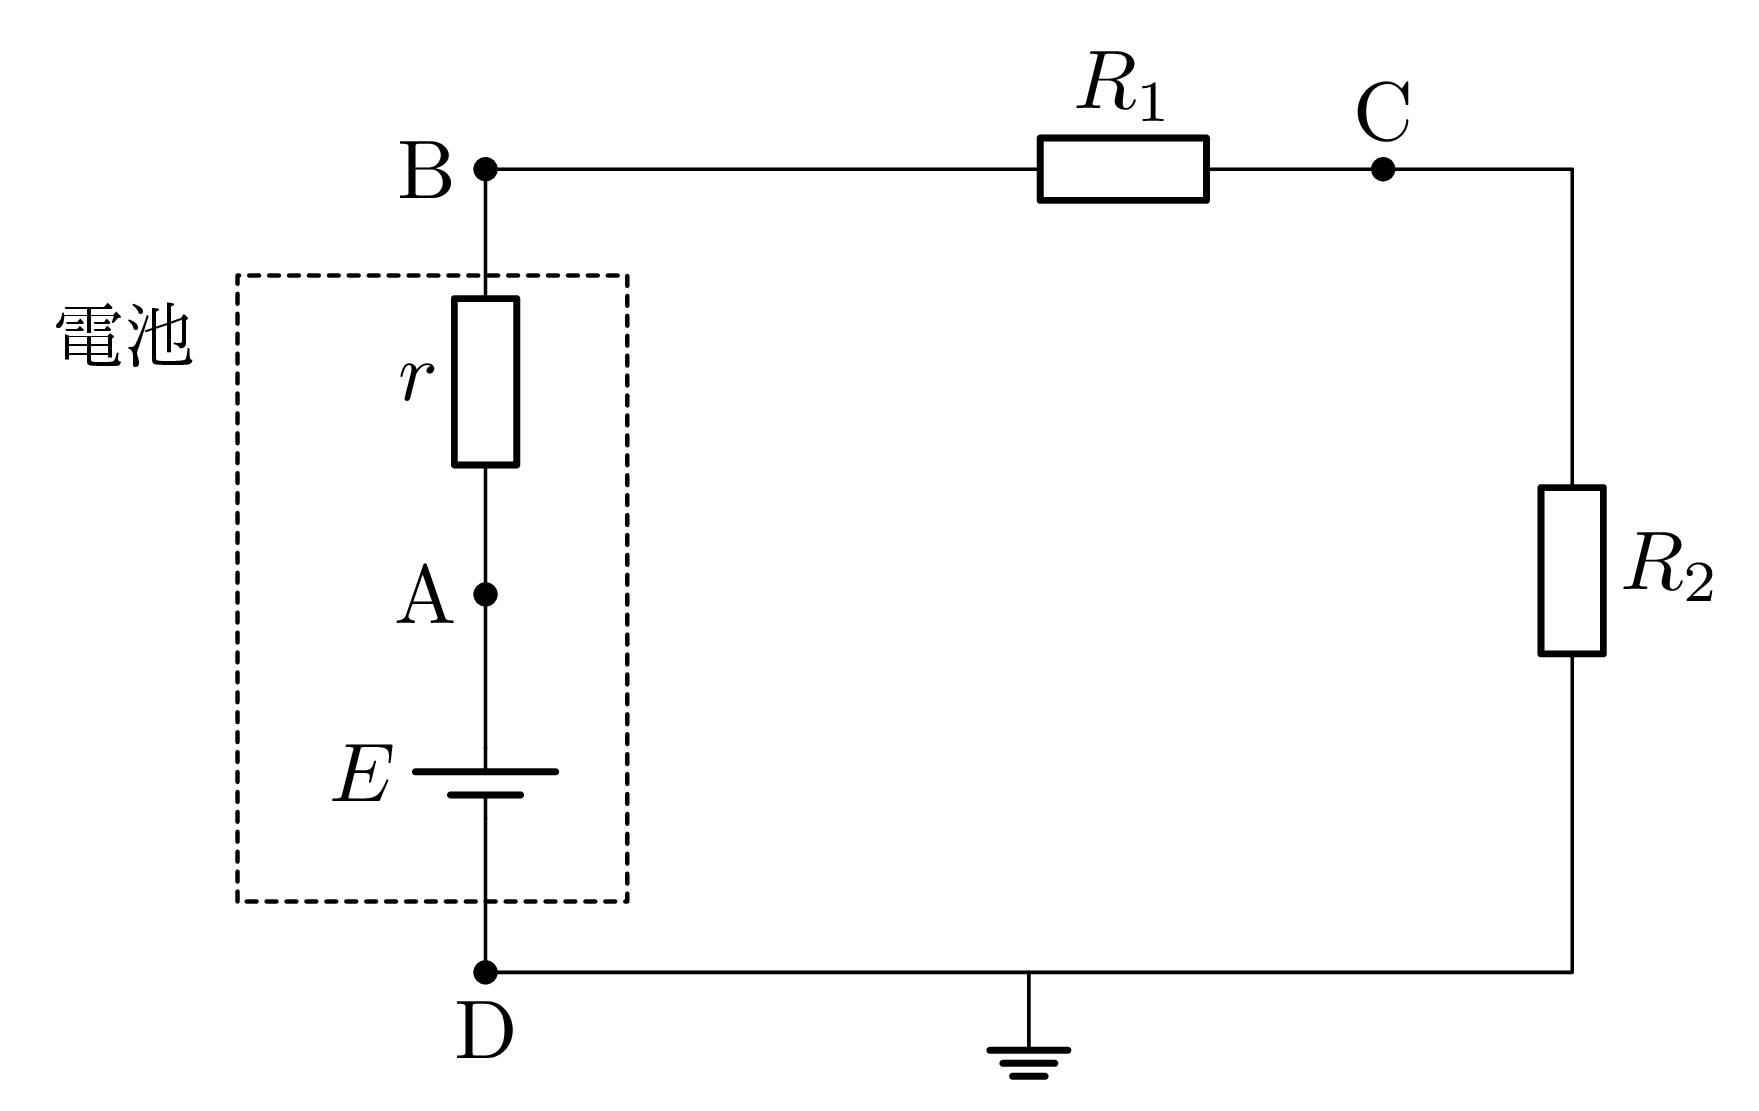
\includegraphics[keepaspectratio,width=58mm]{fig/n26_ex14_zu.png}
\end{zuright}
\end{reidai}

\begin{sisinE}
内部抵抗を電池から分けて描き直すと，起電力$E$と3つの抵抗$r$，$R_1$，$R_2$が直列につながった1本の閉ループになる．
キルヒホッフの第二法則で電流を求めたら，{\gtfamily 接地点$\mathrm{D}$（電位$0$）から出発して，電池では$E$だけ上がり，抵抗では電流の向きに$RI$ずつ下がる}とたどっていけば各点の電位が分かる．
\end{sisinE}

\Key{内部抵抗は電池と分けて描き直す\quad 抵抗では電流の向きに$RI$だけ電位が下がる\quad 接地点の電位は$0$}

\begin{kaitou}
\begin{komon}
\ko{1} 閉ループにキルヒホッフの第二法則を用いると
       \[E=rI+R_1I+R_2I\qquad\therefore\ I=\frac{E}{r+R_1+R_2}\U{A}\Ans\]
\ko{2} $\mathrm{D}$の電位は$0$で，$\mathrm{D}\to\mathrm{A}$では起電力の分だけ電位が上がるので
       \[V_{\mathrm{A}}=E\U{V}\Ans\]
       $\mathrm{A}\to\mathrm{B}$では内部抵抗で$rI$だけ下がるので
       \Ana{V_{\mathrm{B}}=E-rI=\frac{(R_1+R_2)E}{r+R_1+R_2}\U{V}\Ans}
       $\mathrm{B}\to\mathrm{C}$では$R_1$で$R_1I$だけ下がるので
       \[V_{\mathrm{C}}=V_{\mathrm{B}}-R_1I=\frac{R_2E}{r+R_1+R_2}\U{V}\Ans\]
       （$\mathrm{C}\to\mathrm{D}$で$R_2I$下がって$0$に戻ることで検算できる．）
       \begin{center}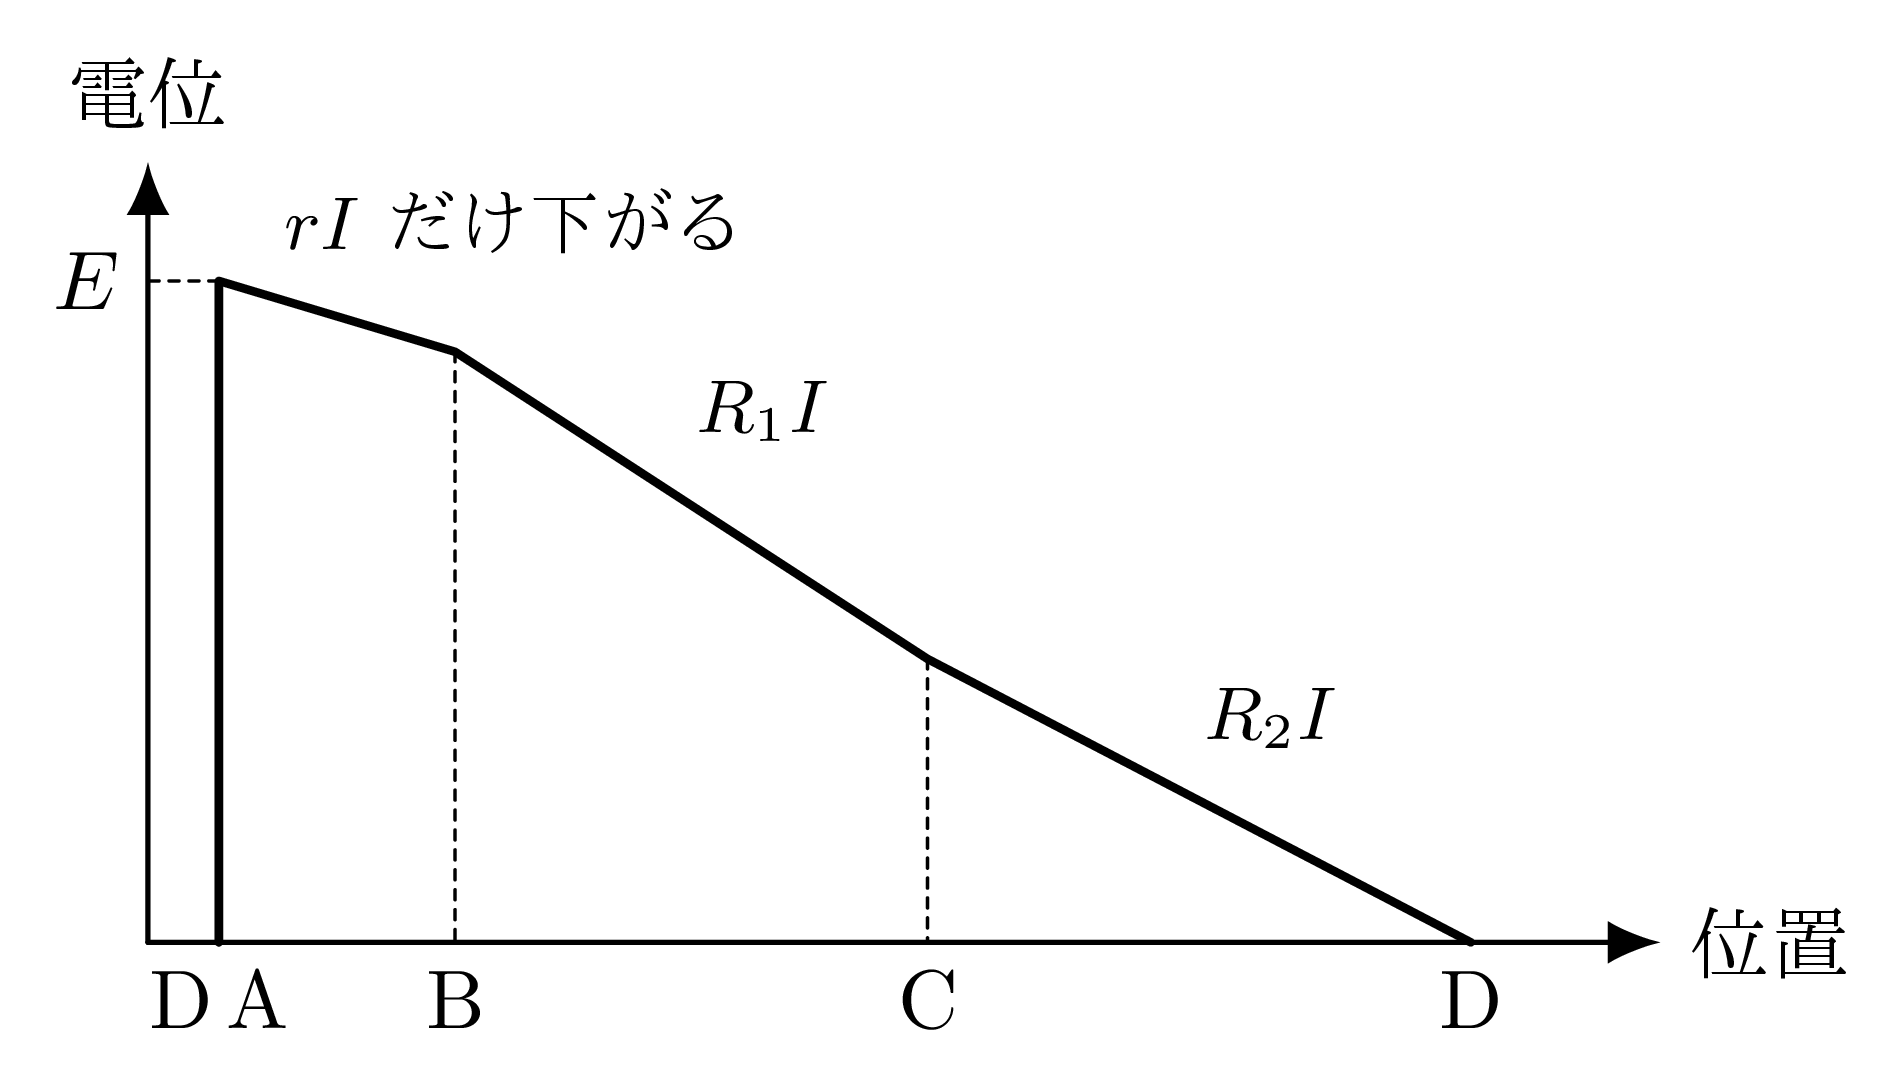
\includegraphics[keepaspectratio,width=62mm]{fig/n26_ex14_ans.png}\end{center}
       \begin{chuu}
       $V_{\mathrm{B}}$が端子電圧である．$V_{\mathrm{B}}=E-rI<E$であり，電流を流すと端子電圧は起電力より小さくなる．
       \end{chuu}
\end{komon}
\end{kaitou}
\end{reidaiunit}

\subsection{電流計と電圧計}

\begin{zuright}{60mm}
\noindent\MARU{1}\ {\gtfamily 電流計}

\hspace{1zw}電流計は，電流の流れる導線が磁場中で受ける力（電磁力，第28回）を利用して電流の大きさを測定する装置であり，電流計を通過していく電流の大きさを測定することができる．
電流計は内部にメーターと，それに直列につながった{\gtfamily 内部抵抗}を持つので，図のように{\gtfamily 内部抵抗とメーターの2つに分けて書き直して考える}とよい（メーター部分の抵抗は$0$とみなす）．

\hspace{1zw}図の点$\mathrm{a}$を流れる電流を測定したい場合には，点$\mathrm{a}$で回路を切って電流計を{\gtfamily 直列に}挿入すればよい．
しかし，電流計の内部抵抗が大きいと，挿入したことで流れる電流そのものが変化してしまう．
そのため，{\gtfamily 電流計の内部抵抗は極めて小さくなければならない}．
\zusep

\includegraphics[keepaspectratio,width=60mm]{text2_p53_fig1.png}
\end{zuright}

\noindent\MARU{2}\ {\gtfamily 電圧計}

電流計の内部抵抗$r\U{\Omega}$が分かっていれば，流れる電流$I\U{A}$から電流計にかかる電圧$V=rI\U{V}$を計算できるから，{\gtfamily 電流計は電圧計として利用することができ}，電流計と電圧計とはほぼ同じ作りになっている．
ただし，測定のしかたと内部抵抗の大きさが異なる．

\begin{center}

\includegraphics[keepaspectratio,width=70mm]{text2_p53_fig2.png}
\end{center}
上図の回路で$\mathrm{ab}$間の電位差を測定したい場合には，$\mathrm{ab}$間に電圧計を{\gtfamily 並列に}接続すればよい．
しかし，電圧計の内部抵抗が小さいと電圧計に電流が流れ込んでしまうため，電流の分布が変わり，測定すべき電位差そのものが変化してしまう．
そのため，{\gtfamily 電圧計の内部抵抗は極めて大きくなければならない}．

% 加筆：分流器・倍率器の定義（原本では例題19 の指針にしか無かった）．
電流計・電圧計には，メーターに流してよい電流の上限（最大目盛り）がある．それ以上の量を測定するには次の工夫をする．
\begin{description}
\item[\MARU{1}\ 分流器] 電流計に{\gtfamily 並列に}小さな抵抗をつなぎ，電流の大部分をそちらへ逃がす．
\item[\MARU{2}\ 倍率器] 電圧計に{\gtfamily 直列に}大きな抵抗をつなぎ，同じ電圧でもメーターに流れる電流を減らす．
\end{description}
どちらも，{\gtfamily メーター部分に流れる電流が上限値を超えないようにするにはどうすればよいか}を考えれば，つなぐ抵抗の値が決まる．

\bsNeed{34mm}
\begin{matome}{電流計・電圧計}
 \hspace{3mm} いずれも{\gtfamily メーター部分と内部抵抗}に分けて描き直す\\
 \hspace{3mm} 電流計：回路に\AnaB{直列}に入れる．内部抵抗は極めて\AnaB{小さい}．\hspace{4mm}分流器は並列につなぐ\\
 \hspace{3mm} 電圧計：回路に\AnaB{並列}に入れる．内部抵抗は極めて\AnaB{大きい}．\hspace{4mm}倍率器は直列につなぐ
\end{matome}

%%%%%%%%%%  例題15（原本の【例題19】）  %%%%%%%%%%%%%%%%%%%%
\bsNeed{56mm}
\begin{reidaiunit}
\begin{reidai}{分流器・倍率器}
\begin{komon}
\ko{1} 内部抵抗が$1.8\U{\Omega}$で，最大$10\U{mA}$まで測定できる電流計がある．これを$100\U{mA}$まで測定できる電流計として用いるためには，何$\U{\Omega}$の抵抗をどのように接続すればよいか．
\ko{2} (1)の結果として，この電流計全体の内部抵抗は何$\U{\Omega}$となるか．
\ko{3} 内部抵抗が$5.0\U{k\Omega}$で，最大$100\U{V}$まで測定できる電圧計がある．これを$500\U{V}$まで測定できる電圧計として用いるためには，何$\U{\Omega}$の抵抗をどのように接続すればよいか．
\ko{4} (3)の結果として，この電圧計全体の内部抵抗は何$\U{\Omega}$となるか．
\ko{5} (1)のはじめの電流計（内部抵抗$1.8\U{\Omega}$，最大$10\U{mA}$）を，最大$1.0\U{V}$まで測定できる電圧計として用いるためにはどのようにすればよいか．
\end{komon}
\end{reidai}

\begin{sisinE}
電流計も電圧計も，メーター部分に流してよい電流の上限が決まっている．
(1)のように，メーターに流れ込む電流を減らすために並列に接続する抵抗が{\gtfamily 分流器}，(3)(5)のように，メーターに流れ込む電流を減らすために直列に接続する抵抗が{\gtfamily 倍率器}である．
いずれも，{\gtfamily 測定したい最大値のときに，メーターにちょうど上限の電流が流れる}ように抵抗値を決める．
\end{sisinE}

\Key{電流計・電圧計はメーター部分と内部抵抗に分けて描く\quad 分流器は並列\quad 倍率器は直列}

\begin{kaitou}
\begin{komon}
\ko{1} 全体に$100\U{mA}$が流れ込んだとき，電流計（内部抵抗$1.8\U{\Omega}$）にちょうど$10\U{mA}$が流れ，残りの$90\U{mA}$が並列につないだ抵抗$R_{\mathrm{s}}$に流れればよい．並列部分の電圧は等しいので
       \begin{center}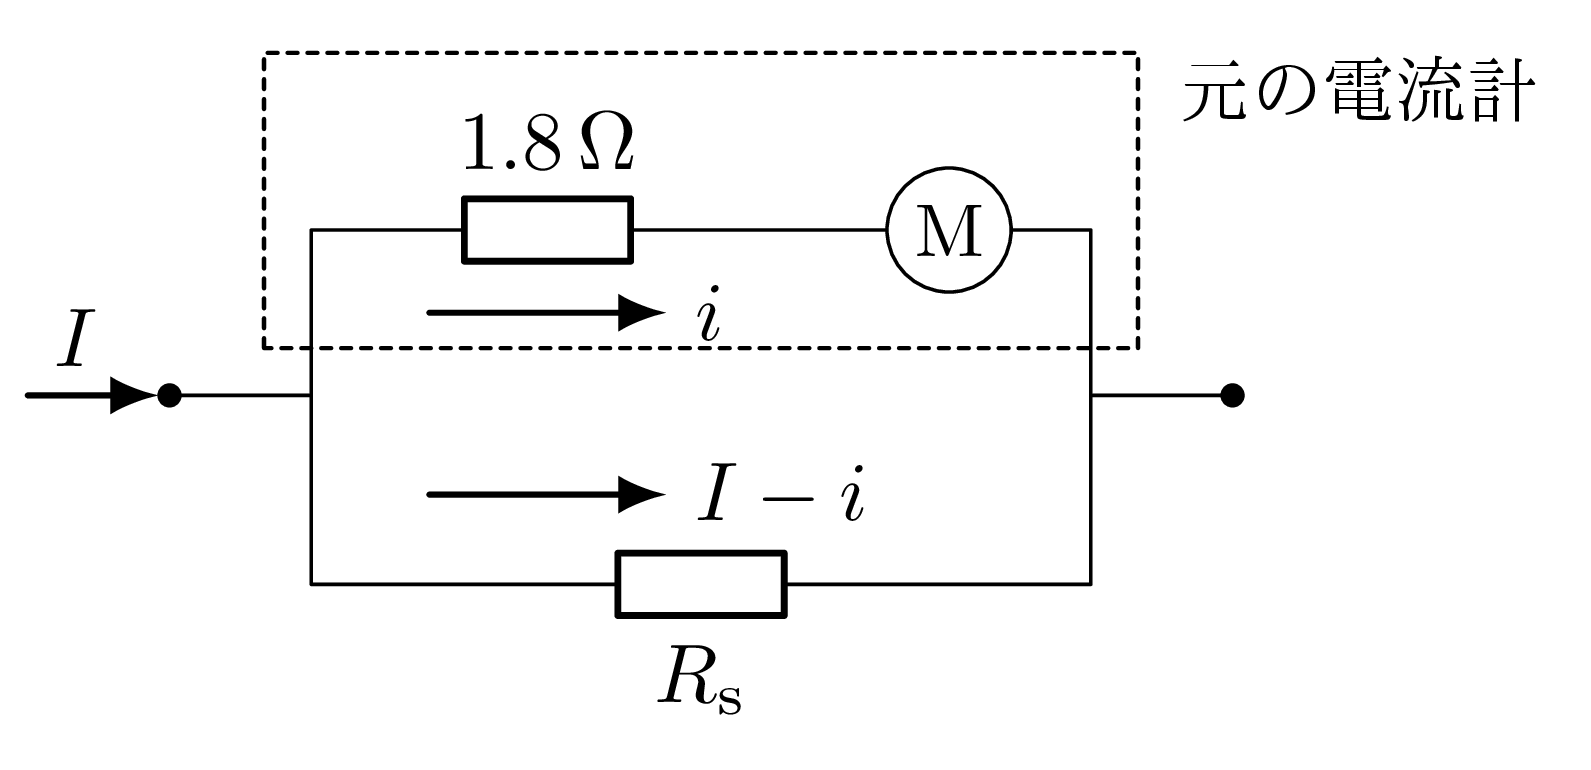
\includegraphics[keepaspectratio,width=60mm]{fig/n26_ex15_ans1.png}\end{center}
       \Ana{1.8\times 10\times 10^{-3}=R_{\mathrm{s}}\times 90\times 10^{-3}\qquad\therefore\ R_{\mathrm{s}}=0.20\U{\Omega}}
       よって，{\gtfamily $0.20\U{\Omega}$の抵抗を電流計に並列に}接続すればよい．\Ans
\ko{2} $1.8\U{\Omega}$と$0.20\U{\Omega}$の並列なので
       \[\Bigl(\frac{1}{1.8}+\frac{1}{0.20}\Bigr)^{-1}=0.18\U{\Omega}\Ans\]
\ko{3} この電圧計は$100\U{V}$のとき$\dfrac{100}{5.0\times 10^3}=2.0\times 10^{-2}\U{A}$の電流が流れて最大目盛りを指す．$500\U{V}$をかけたときに同じ電流が流れるように，直列に抵抗$R_{\mathrm{m}}$をつなぐ：
       \begin{center}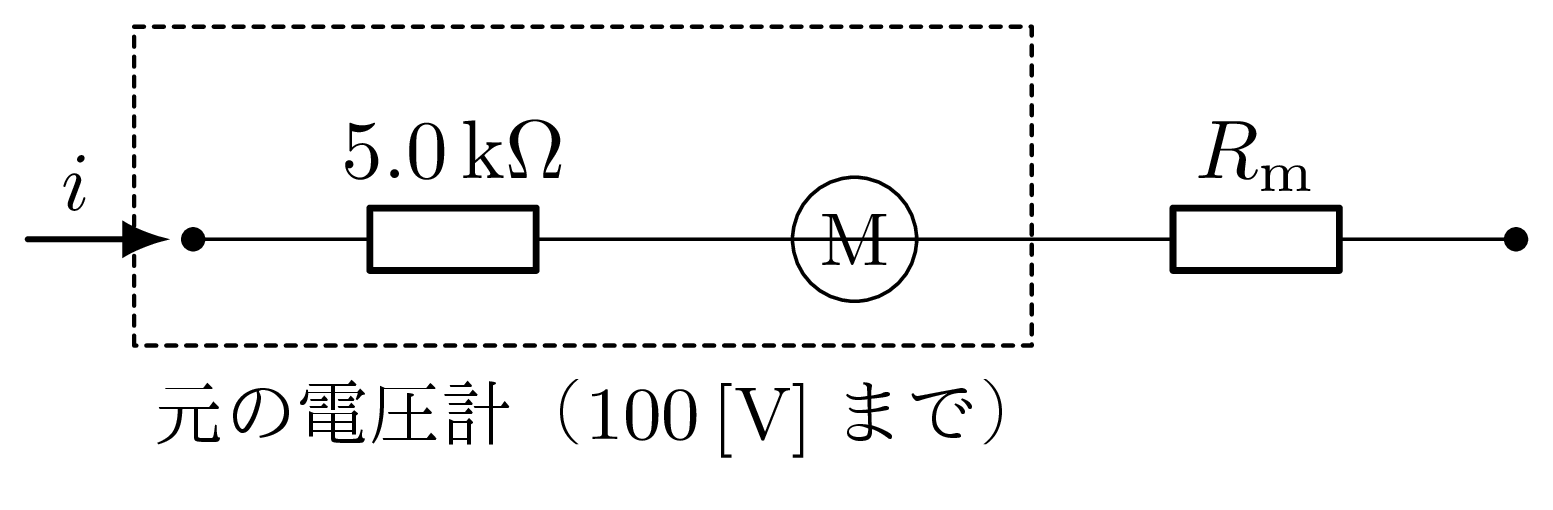
\includegraphics[keepaspectratio,width=60mm]{fig/n26_ex15_ans2.png}\end{center}
       \Ana{500=(5.0\times 10^3+R_{\mathrm{m}})\times 2.0\times 10^{-2}\qquad\therefore\ R_{\mathrm{m}}=2.0\times 10^4\U{\Omega}}
       よって，{\gtfamily $2.0\times 10^4\U{\Omega}$（$20\U{k\Omega}$）の抵抗を電圧計に直列に}接続すればよい．\Ans
\ko{4} $5.0\U{k\Omega}$と$20\U{k\Omega}$の直列なので
       \[2.5\times 10^4\U{\Omega}\Ans\]
\ko{5} $1.0\U{V}$をかけたときにちょうど$10\U{mA}$が流れるように，直列に抵抗$R$をつなぐ：
       \[1.0=(1.8+R)\times 10\times 10^{-3}\qquad\therefore\ R=98.2\U{\Omega}\]
       よって，{\gtfamily $98.2\U{\Omega}$の抵抗を電流計に直列に}接続すればよい．\Ans
       \begin{chuu}
       もとの電流計のままでも，最大$1.8\times 10\times 10^{-3}=1.8\times 10^{-2}\U{V}$までの電圧計として使える．直列に抵抗を足すことで，測れる電圧の範囲を広げたのである．電流計と電圧計が「ほぼ同じ作り」であることがよく分かる．
       \end{chuu}
\end{komon}
\end{kaitou}
\end{reidaiunit}

% 加筆（2026-09-24）：練習［60］(7)（ブリッジの平衡）と［68］（立方体）の前提．
%   原本では ㉞34.4 にブリッジの結論だけ，対称性の使い方は［41］の解答にしか無かった．
%   ブリッジの系統的な扱い（メートルブリッジ・ポテンシオメータ）は第27回．
\subsection{回路を整理するための2つの着眼点}

複雑に見える回路も，次の2つに着目すると直列・並列の組み合わせに書き直せることがある．

\noindent\MARU{1}\ {\gtfamily 等電位の2点の間には電流が流れない}

電位差が$0$の2点の間に抵抗や検流計があっても，そこには電流が流れない（$I=\dfrac{V}{R}=0$）．
したがって，{\gtfamily 等電位の2点を結ぶ導線は，外してもつないでも回路の他の部分の電流は変わらない}．

\begin{zuright}{44mm}
\hspace{1zw}右図の回路（{\gtfamily ホイートストンブリッジ}）で，$\mathrm{A}\to\mathrm{B}\to\mathrm{D}$と$\mathrm{A}\to\mathrm{C}\to\mathrm{D}$の2つの道筋を考える．
検流計$\mathrm{G}$に電流が流れていなければ，$R_1$と$R_3$には同じ電流$I_1$が，$R_2$と$R_4$には同じ電流$I_2$が流れる．
$\mathrm{B}$と$\mathrm{C}$が等電位であることから，$\mathrm{A}$からの電圧降下が等しく，$\mathrm{D}$までの電圧降下も等しい：
\[R_1I_1=R_2I_2,\qquad R_3I_1=R_4I_2\]
辺々割れば
\zusep

\includegraphics[keepaspectratio,width=44mm]{text2_p55_fig1.png}
\end{zuright}
\AnaBD{R_1:R_2=R_3:R_4\quad(R_1R_4=R_2R_3)}
が得られる．これを{\gtfamily ブリッジの平衡条件}という．
逆に，この条件が成り立っていれば$\mathrm{B}$，$\mathrm{C}$は等電位なので，$\mathrm{G}$には電流が流れない．
ブリッジを使った抵抗の測定は第27回で扱う．

\noindent\MARU{2}\ {\gtfamily 対称な回路では電流の分布も対称になる}

回路が電流の入口と出口を結ぶ線に関して対称であれば，対称な位置にある抵抗には同じ大きさの電流が流れる．
対称な位置にある点どうしは等電位になるので，\MARU{1}と組み合わせて「電流の流れない導線」を見つけることができる．
さらに，{\gtfamily 電池の向きを逆にすると，すべての電流は大きさが同じまま向きだけが逆になる}ことを使うと，入口と出口を入れかえた対称性まで利用できる（練習［68］）．

\newpage

%%%%%%%%%%%%%%%%%%%%  練習問題  %%%%%%%%%%%%%%%%%%%%
% 第25回の［59］に続く．
\setcounter{qno}{59}

\filbreak
\Rank{A問題}

% A問題の統合（再編案の「A2→1」）：旧㉝[29]（(1)〜(4)）と旧㉞[36]（(1)〜(3)）を1題にまとめた．
%   設問は1つも失われていない（(5)〜(7) が旧㉞[36] の(1)〜(3)）．
\Mon{基本公式の確認}

\hspace{1zw}以下の設問に答えよ．
\begin{komon}
\ko{1} ある抵抗に$0.20\U{A}$の電流が$40\U{s}$間流れた．抵抗を通過した電気量は何$\U{C}$か．
\ko{2} $52\U{\Omega}$の抵抗の両端に$13\U{V}$の電圧をかけたとき，この抵抗を流れる電流の強さは何$\U{A}$か．
\ko{3} 断面積$2.0\times 10^{-6}\U{m^2}$，長さ$30\U{m}$の銅線がある．この銅線の抵抗値は何$\U{\Omega}$か．ただし，銅の抵抗率を$1.7\times 10^{-8}\U{\Omega\cdot m}$とする．
\ko{4} $20\U{\Omega}$の抵抗に強さ$3.0\U{A}$の電流を流したとき，この抵抗における消費電力は何$\U{W}$か．
\end{komon}
\begin{zuright}{60mm}
\begin{komon}
\ko{5} 右図は回路の一部であり，図のように電流が流れていた．この電池の起電力は何$\U{V}$か．ただし，電池の内部抵抗は無視してよい．
\ko{6} 抵抗値$2.0\U{\Omega}$と$3.0\U{\Omega}$の抵抗を直列につないだときの合成抵抗は何$\U{\Omega}$か．またこれらを並列につないだときの合成抵抗は何$\U{\Omega}$か．
\end{komon}
\zusep
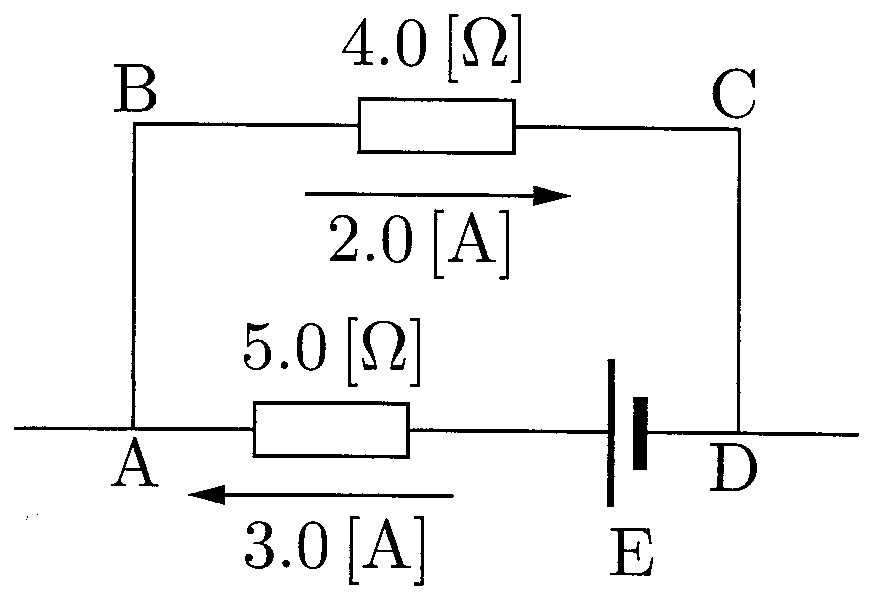
\includegraphics[keepaspectratio,width=56mm]{fig/n26_p60_zu1.png}
\end{zuright}
\begin{zuright}{50mm}
\begin{komon}
\ko{7} 右図の回路では検流計$\mathrm{G}$には電流が流れていない．このとき抵抗$\mathrm{R}$の抵抗値は何$\U{\Omega}$か．
\end{komon}
\zusep
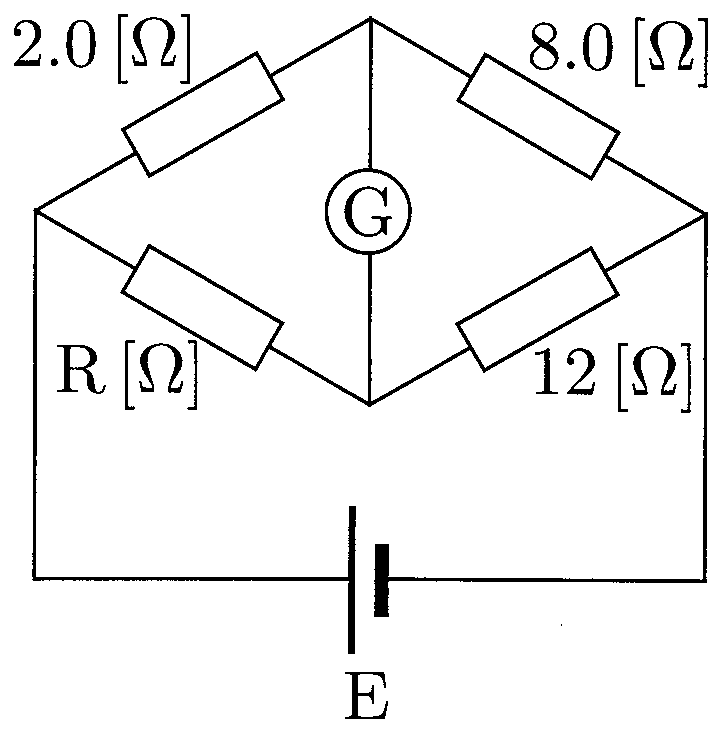
\includegraphics[keepaspectratio,width=46mm]{fig/n26_p60_zu2.png}
\end{zuright}

\filbreak
\Rank{B問題}

\Mon{電流と電荷の移動の関係}

\hspace{1zw}切り口の面積が$1.0\U{mm^2}$の針金に，$2.0\U{A}$の電流が流れている．このとき，針金内の自由電子が全体として移動する平均の速さを求めよ．ただし，この針金の$1\U{m^3}$あたりの自由電子の個数を$8.5\times 10^{28}$個とし，電子の電荷は$-1.6\times 10^{-19}\U{C}$である．

\Mon[\Sitei]{オームの法則}

\hspace{1zw}長さ$l_0\U{m}$，断面積$S_0\U{m^2}$の抵抗に，内部抵抗の無視できる起電力$V_0\U{V}$の電池をつないだところ，この抵抗には強さ$I_0\U{A}$の電流が流れた．これについて以下の設問に答えよ．
\begin{komon}
\ko{1} 抵抗の長さおよび断面積をそのままに保ったまま電池の起電力を$kV_0\U{V}$にしたとき，抵抗に流れる電流の強さを求めよ．
\ko{2} 電池の起電力を$V_0\U{V}$のままに保ったまま，抵抗の長さを$kl_0\U{m}$にしたとき，抵抗に流れる電流の強さを求めよ．
\ko{3} 電池の起電力をそのままに保ったまま，抵抗の断面積を$kS_0\U{m^2}$にしたとき，抵抗に流れる電流の強さを求めよ．
\end{komon}

\Mon[\Sitei]{電気抵抗の加速モデル}

\hspace{1zw}電気抵抗が生じる理由は，導体中を移動する電子が陽イオンに衝突して抵抗を受けるためである．陽イオンへの衝突を，陽イオンから，電子の持つ速度と逆向きに，速さに比例した抵抗力を受けるとみなして電気抵抗を導く方法があるが（例題12），これは少し大ざっぱなモデルである．実際には自由電子は常に陽イオンから抵抗力を受けているのではなく，導体にかけた電圧によって加速されて等加速度運動を行ってある程度の時間だけ加速される．しかしそのあと陽イオンとの衝突によって減速し，また再び加速していく，ということを繰り返していると考えられる．これを少し簡単化して，電気抵抗が生じる原因を考えてみよう．以下の文の空欄に適当な語句または式を当てはめよ．
\begin{center}
\begin{minipage}[t]{62mm}\centering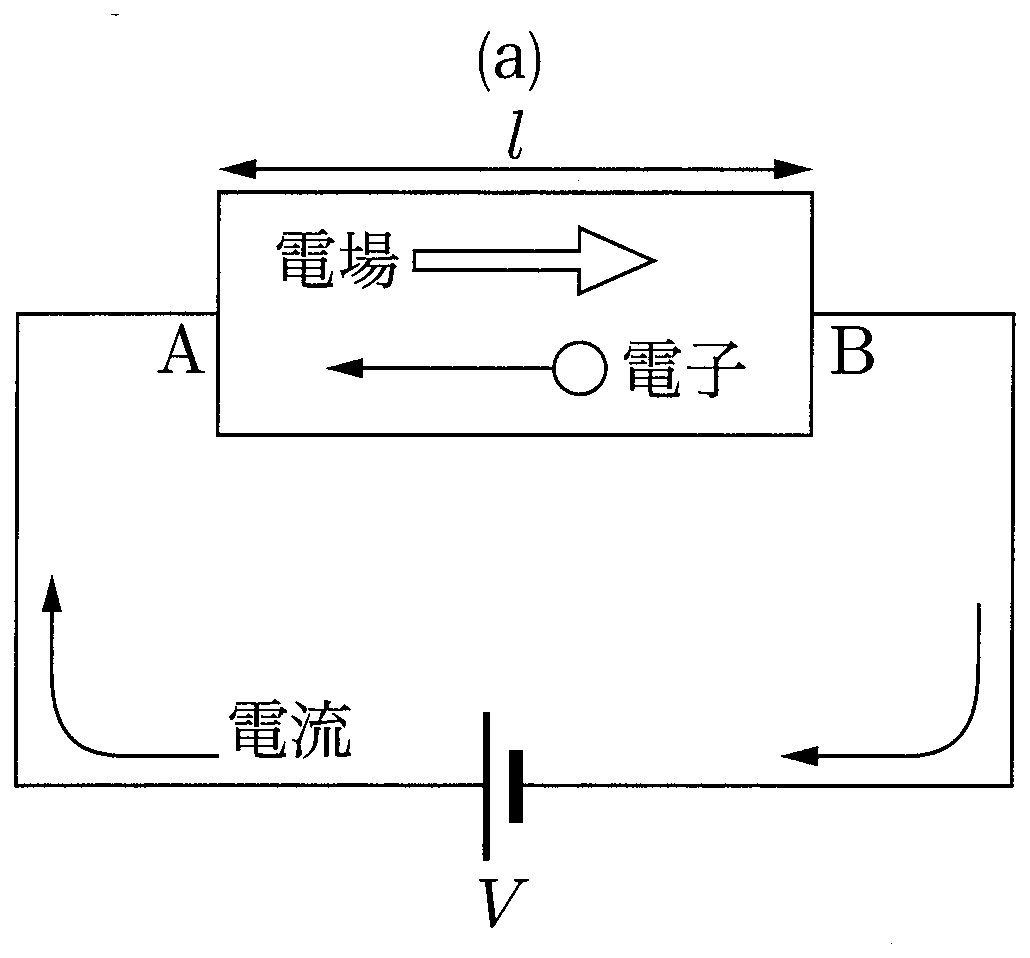
\includegraphics[keepaspectratio,width=52mm]{fig/n26_p63_a.png}\end{minipage}\hspace{4mm}%
\begin{minipage}[t]{62mm}\centering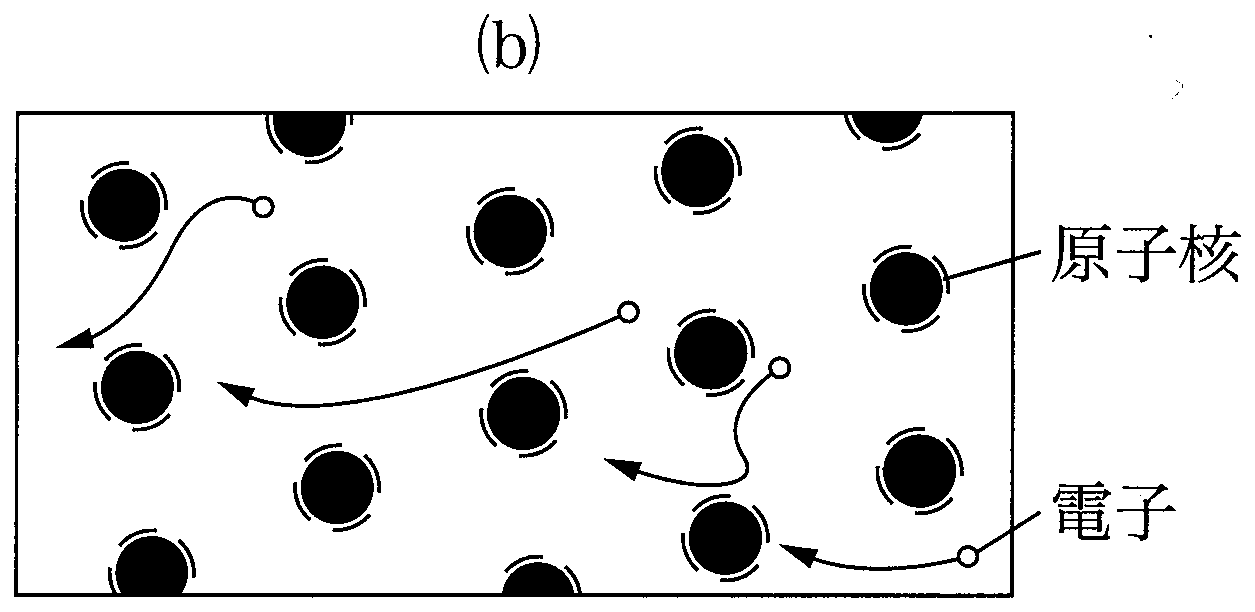
\includegraphics[keepaspectratio,width=62mm]{fig/n26_p63_b.png}\end{minipage}\\[3mm]
\begin{minipage}[t]{62mm}\centering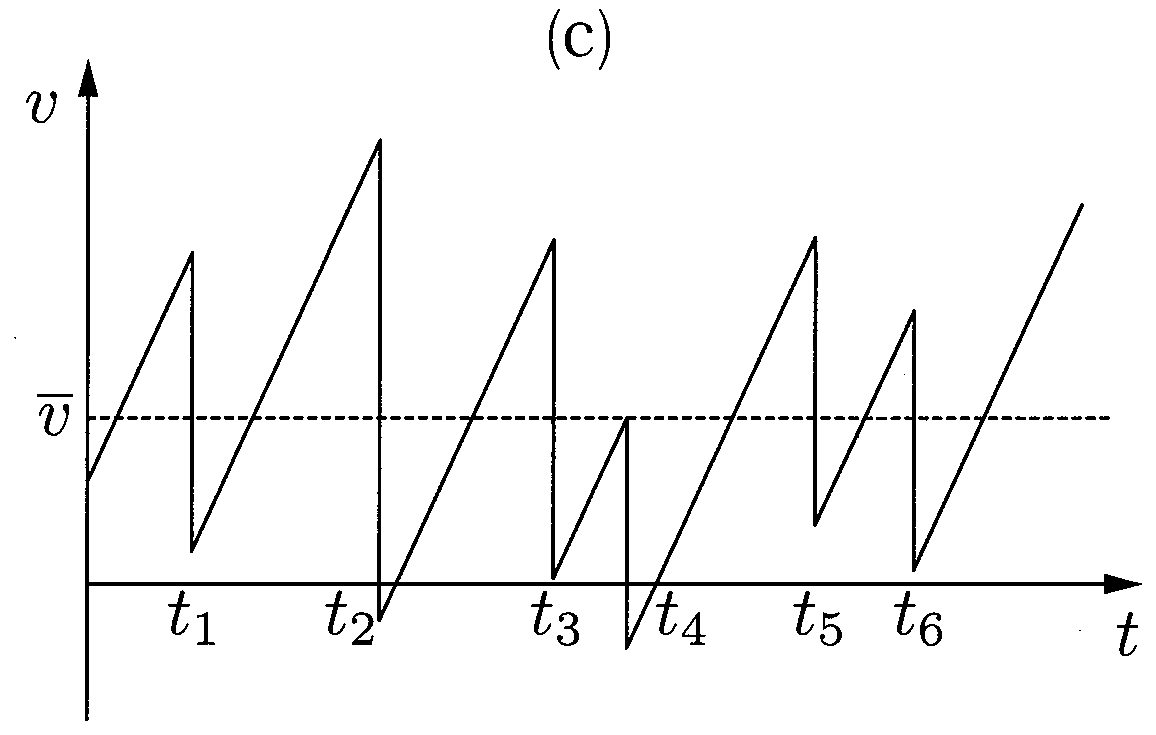
\includegraphics[keepaspectratio,width=58mm]{fig/n26_p63_c.png}\end{minipage}\hspace{4mm}%
\begin{minipage}[t]{62mm}\centering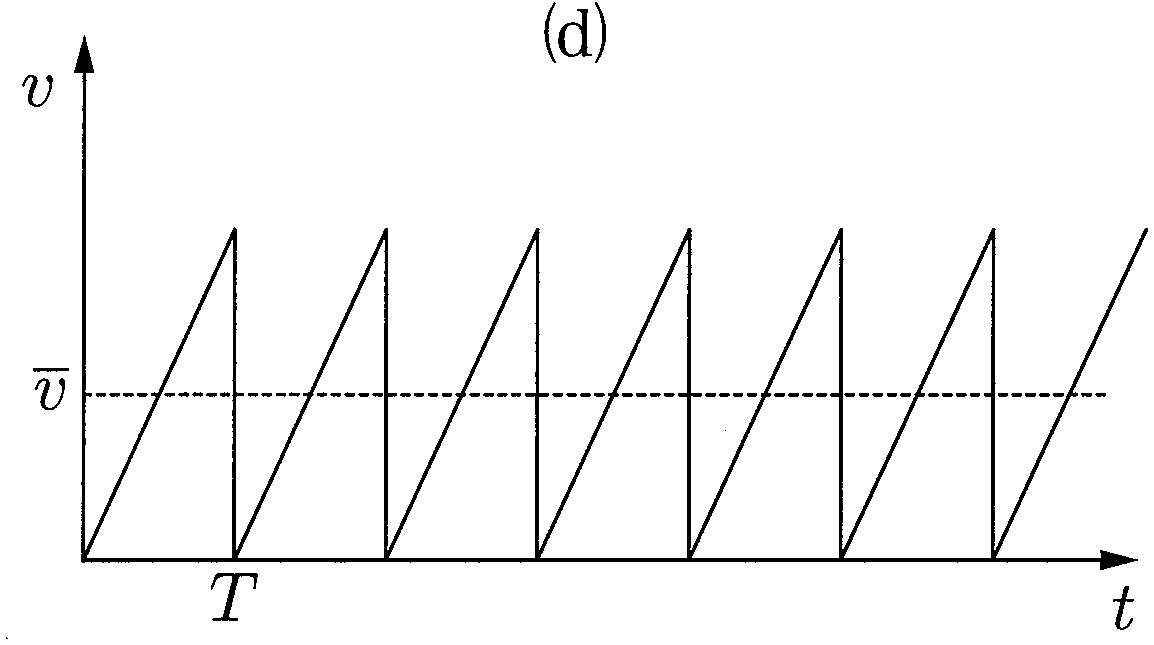
\includegraphics[keepaspectratio,width=58mm]{fig/n26_p63_d.png}\end{minipage}
\end{center}
\hspace{1zw}図(a)のように，長さ$l\U{m}$，断面積$S\U{m^2}$，自由電子の密度が$n\U{個/m^3}$の金属棒に対して，電圧$V\U{V}$の電池を接続する．このとき，金属棒内には$\mathrm{A}$から$\mathrm{B}$向きに大きさ\framebox[4zw]{\rule{0pt}{1.1zw}1}の電場が生じるため，電子は左向きに力を受ける．自由電子（質量$m\U{kg}$，電荷$-e\U{C}$）の左向きの加速度を$a\U{m/s^2}$とすると，この電子の運動方程式は\framebox[4zw]{\rule{0pt}{1.1zw}2}であるから，その加速度は\framebox[4zw]{\rule{0pt}{1.1zw}3}であり，これより各自由電子は等加速度運動をすることになる．しかし各自由電子はごく短い時間（金属の種類によって変わるが，$10^{-12}\sim 10^{-15}$秒程度）加速された後，金属棒を構成する原子に衝突し，等加速度運動で得られた速度を失い，そしてまた加速される．これは実際には図(b)のように起こるため，自由電子の持つ，$\mathrm{B}$から$\mathrm{A}$向きの速さは図(c)のように乱雑に変化するが，簡単のため，図(d)のように自由電子は等しい時間間隔$T\U{s}$で原子に衝突し，そして衝突時に等加速度運動で得られた速度のすべてを失い，そして，また加速され衝突することを繰り返すと考えよう．
\par
\hspace{1zw}このように考えると，各自由電子が陽イオンに衝突する直前の速さは\framebox[4zw]{\rule{0pt}{1.1zw}4}であり，$\mathrm{B}$から$\mathrm{A}$向きの電子の平均的な速さ$\overline{v}$は\framebox[4zw]{\rule{0pt}{1.1zw}5}となる．よって，電圧$V\U{V}$の電池を接続したときにこの金属棒に流れる電流の強さは\framebox{\rule{0pt}{1.1zw}\,6（$e$，$n$，$T$，$S$，$m$，$l$，$V$で表せ）\,}であるから，これより流れる電流の強さはかけた電圧の大きさに比例する．よってこの金属棒の電気抵抗値は\framebox[4zw]{\rule{0pt}{1.1zw}7}であり，これは断面積の\framebox{\rule{0pt}{1.1zw}\,8（○乗に\{比例 or 反比例\}）\,}し，導線の長さの\framebox{\rule{0pt}{1.1zw}\,9（○乗に\{比例 or 反比例\}）\,}しているので，このモデルは現実に即していると言える．
\par
\hspace{1zw}また，一個の自由電子は衝突によって静止するので，一回の衝突によって原子に与えるエネルギーは\framebox[4zw]{\rule{0pt}{1.1zw}10}である．金属棒内の自由電子の総数が\framebox[4zw]{\rule{0pt}{1.1zw}11}であること，および一個の自由電子は$1\U{s}$間あたりに\framebox[4zw]{\rule{0pt}{1.1zw}12}回だけ衝突することに注意すると，自由電子全体で$1\U{s}$間に金属棒の原子に与える全エネルギーは\framebox[4zw]{\rule{0pt}{1.1zw}13}となる．このエネルギーが金属棒からジュール熱として放出されるので，金属から放出される単位時間あたりのジュール熱は，流れている電流の強さ$I\U{A}$およびかけた電圧$V\U{V}$を用いて，\framebox[4zw]{\rule{0pt}{1.1zw}14}と表される．

\Mon{抵抗の温度変化}

\begin{zuright}{44mm}
\hspace{1zw}温度が$t_1$，$t_2\U{^\circ C}$のときの抵抗値がそれぞれ$R_1$，$R_2\U{\Omega}$である物質がある．
\begin{komon}
\ko{1} この物質の$0\U{^\circ C}$における抵抗値$R_0\U{\Omega}$および抵抗率の温度係数$\alpha\U{/K}$を求めよ．ただしこの物質の抵抗値は温度に対して直線的に増加するものとする．
\ko{2} この物質に対してかけた電圧とそのとき流れた電流をグラフにしたところ，右図のようなグラフが得られた．この物質の温度係数の正負を答えよ．またこの物質は，\MARU{1}金属，\MARU{2}半導体のいずれか．理由も述べよ．
\end{komon}
\zusep
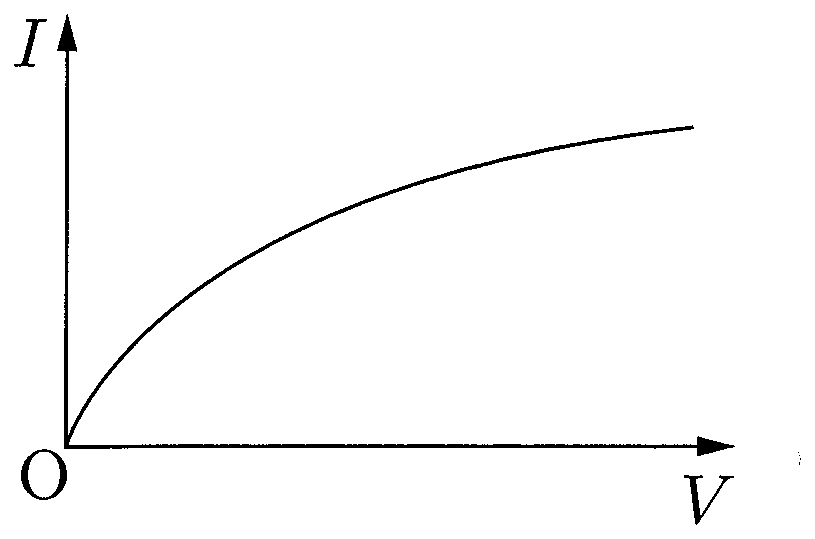
\includegraphics[keepaspectratio,width=40mm]{fig/n26_p64_zu.png}
\end{zuright}

\Mon{電流計・電圧計}

\begin{zuright}{50mm}
\hspace{1zw}今，図(a)(b)のような回路によって，抵抗の抵抗値$R\U{\Omega}$，電流計の内部抵抗の抵抗値$r_{\mathrm{A}}\U{\Omega}$，電圧計の内部抵抗の抵抗値$r_{\mathrm{V}}\U{\Omega}$を求める実験を行う．図(a)のようにつないで実験を行ったところ，電圧計および電流計の読みはそれぞれ$v_a=4.92\U{V}$，$i_a=0.540\U{A}$と読み取られ，また図(b)のようにつないで実験を行ったところ，電圧計および電流計の読みはそれぞれ$v_b=6.00\U{V}$，$i_b=0.500\U{A}$と読み取られた．電池の内部抵抗が無視できるとき，これらのことを用いて，この電池の起電力，抵抗の抵抗値$R\U{\Omega}$，電流計の内部抵抗の抵抗値$r_{\mathrm{A}}\U{\Omega}$，電圧計の内部抵抗の抵抗値$r_{\mathrm{V}}\U{\Omega}$を求めよ．
\zusep
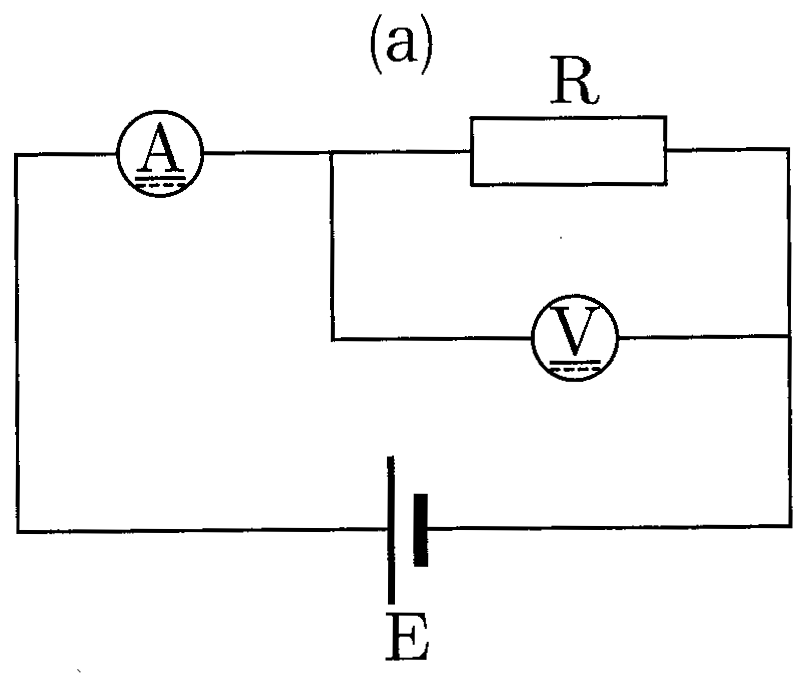
\includegraphics[keepaspectratio,width=46mm]{fig/n26_p65_a.png}\\[2mm]
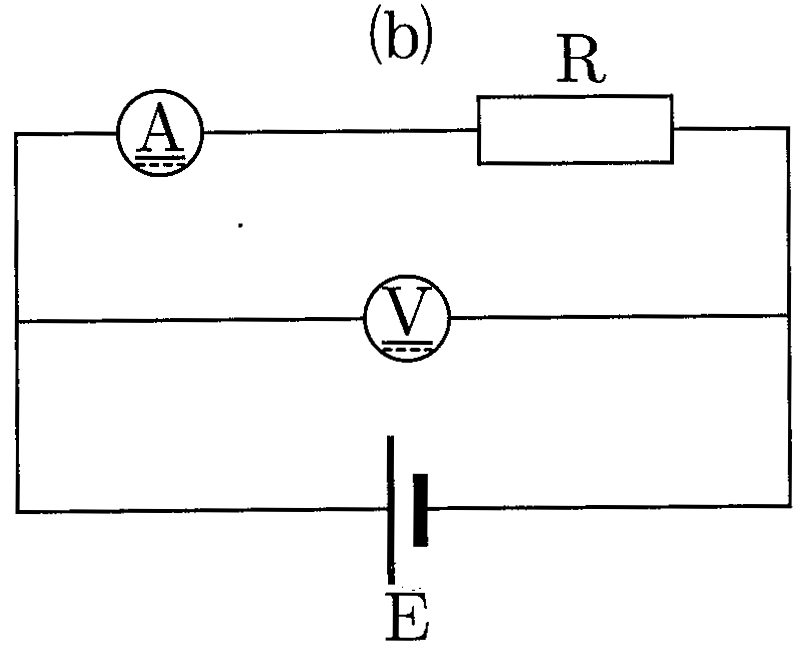
\includegraphics[keepaspectratio,width=46mm]{fig/n26_p65_b.png}
\end{zuright}

\filbreak
\Rank{C問題}

\Mon{すべり抵抗}

\begin{zuright}{56mm}
\hspace{1zw}右図に示した回路において，$\mathrm{AB}$は全長$l\U{m}$，全抵抗値$R_0\U{\Omega}$のすべり抵抗であり，$\mathrm{AC}$，$\mathrm{CB}$間の抵抗値は，それぞれ$\mathrm{AC}$，$\mathrm{CB}$間の長さに比例する．また電池$\mathrm{E}$の起電力は$E\U{V}$であり，$\mathrm{D}$は抵抗値$R_0\U{\Omega}$の抵抗であるとして以下の設問に答えよ．ただし電池の内部抵抗は無視できるものとし，$\mathrm{AC}=x\U{m}$とする．
\zusep
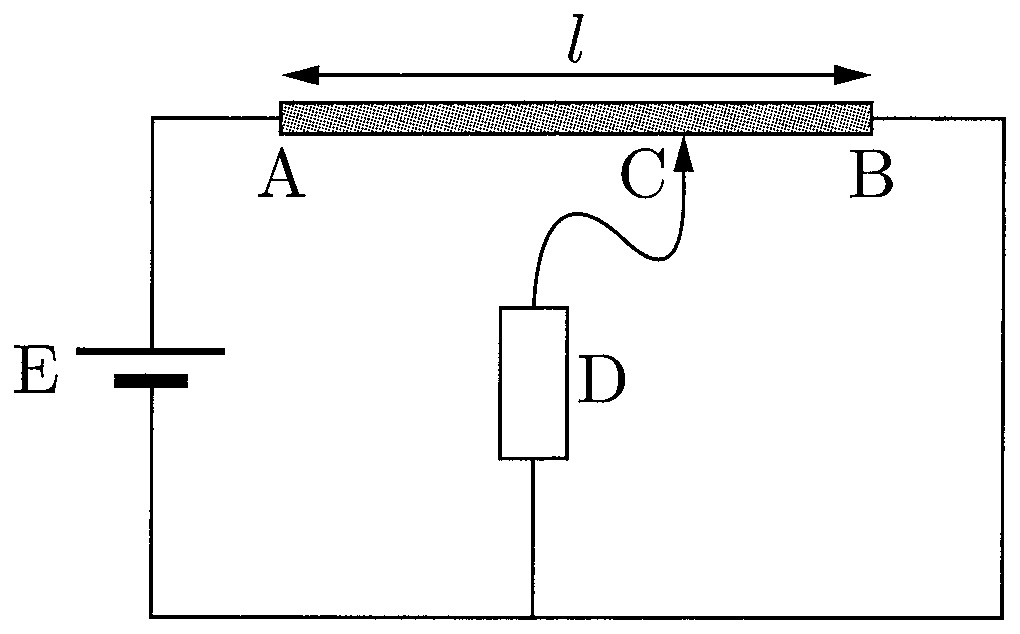
\includegraphics[keepaspectratio,width=56mm]{fig/n26_p66_zu.png}
\end{zuright}
\begin{komon}
\ko{1} $\mathrm{D}$を下向きに流れる電流の強さを$I(x)\U{A}$，$\mathrm{CB}$を右向きに流れる電流の強さを$i(x)\U{A}$とする．このとき，$\mathrm{A}$から$\mathrm{C}$に流れ込む電流は，そのあと$\mathrm{B}$，$\mathrm{D}$側にそれぞれ分流するため，$I(x)+i(x)\U{A}$になっている．このこととキルヒホッフの第二法則を用いて回路に成り立つ式を立てよ．
\ko{2} $i(x)\U{A}$を求め，これが最小となるような$x$の値$x_0\U{m}$を求めよ．
\end{komon}

\Mon{電池の内部抵抗}

\hspace{1zw}内部抵抗$r\U{\Omega}$，起電力$V\U{V}$の電池に抵抗値$R\U{\Omega}$の外部抵抗を接続した．以下の設問に答えよ．
\begin{komon}
\ko{1} このとき回路を流れる電流の強さ$I\U{A}$を求めよ．
\ko{2} 外部抵抗で消費する電力$P\U{W}$を求め，これが最大となるような外部抵抗の値を求めよ．
\end{komon}

\Mon{合成抵抗}

\begin{zuright}{46mm}
\hspace{1zw}抵抗値$r\U{\Omega}$を持つ直線抵抗を何本か用意し，この両端をうまくつなぎあわせて図のような立方体を作った．今，$\mathrm{a}$，$\mathrm{c}$間に電池を接続して流れたときの電流を考える．このとき，回路の対称性をうまく利用して，以下の設問に答えよ．
\begin{komon}
\ko{1} この図のうち，二つの抵抗線を外しても$\mathrm{a}$，$\mathrm{c}$間の合成抵抗に変化はない．この二つの抵抗はどの辺とどの辺の抵抗か．理由を付けて答えよ．
\ko{2} $\mathrm{a}$，$\mathrm{c}$間の合成抵抗を求めよ．
\end{komon}
\zusep
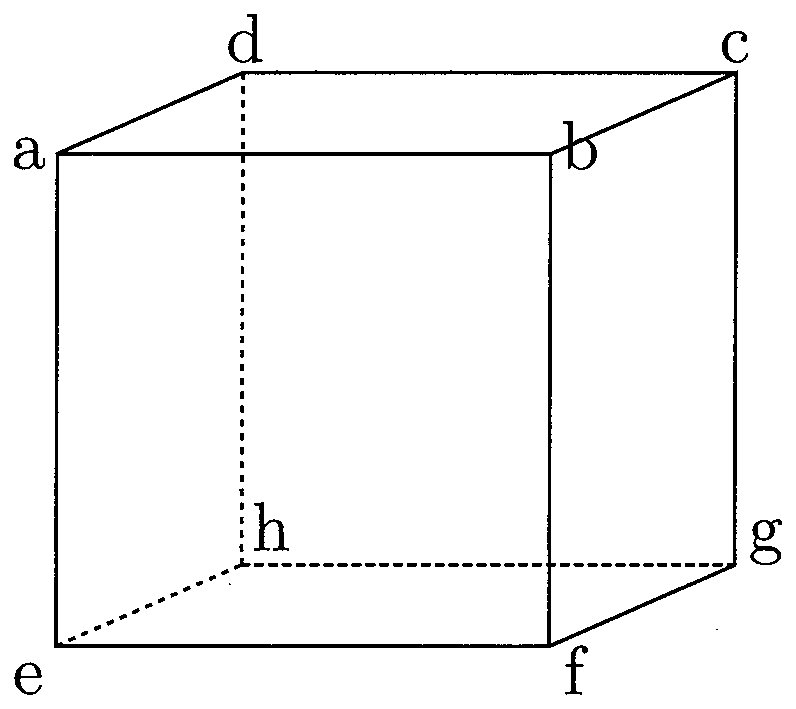
\includegraphics[keepaspectratio,width=44mm]{fig/n26_p68_zu.png}
\end{zuright}

\newpage

%%%%%%%%%%%%%%%%%%%%  解答  %%%%%%%%%%%%%%%%%%%%
\KaiTitle{第26回　電流・電気抵抗・抵抗の接続と計器}
\setlength{\columnseprule}{0.4pt}
\begin{multicols}{2}
\raggedcolumns

\Rank{A問題}
\MonN{60}{基本公式の確認}\par\nopagebreak
\begin{sisin}
(1)〜(4) $Q=I\cdot\varDelta t$，$V=RI$の関係式はよいだろうが，抵抗率の定義式$R=\rho\dfrac{l}{S}\U{\Omega}$および抵抗率の単位$\rho\U{\Omega\cdot m}$に注意せよ．抵抗率の式中の$S$，$l$の分母・分子を逆にしないようにきちんと覚えておこう．直観的に考えて，抵抗が短いほど，また断面積が大きいほど電流は流れやすくなるはずなので抵抗値は小さくなるはず．そう考えれば，$l$は分子，$S$は分母に来ることが分かる．

(5)については各抵抗における電圧降下の大きさおよび向きをよく考え，ループに対してキルヒホッフの第二法則を立てればよい．(6)(7)については合成抵抗の公式とブリッジの平衡条件（26.9）を利用して処理しよう．
\end{sisin}
\KaiHead
\begin{komon}
\ko{1} \[Q=I\cdot\varDelta t=0.20\times 40=8.0\U{C}\Ans\]
\ko{2} $V=RI$より，
       \[I=\frac{V}{R}=\frac{13}{52}=0.25\U{A}\Ans\]
\ko{3} \[\begin{aligned}
         R&=\rho\frac{l}{S}=1.7\times 10^{-8}\times\frac{30}{2.0\times 10^{-6}}\\
          &\fallingdotseq 0.26\U{\Omega}\Ans
       \end{aligned}\]
\ko{4} \[P=RI^2=20\times 3.0^2=180\U{W}\Ans\]
\ko{5} 電池の起電力を$V\U{V}$として，閉回路$\mathrm{ABCDA}$についてキルヒホッフの第二法則より立式すると，
       \[V=5.0\times 3.0+4.0\times 2.0\]
       ゆえ，これを解いて，
       \[V=2.3\times 10\U{V}\Ans\]
       \begin{center}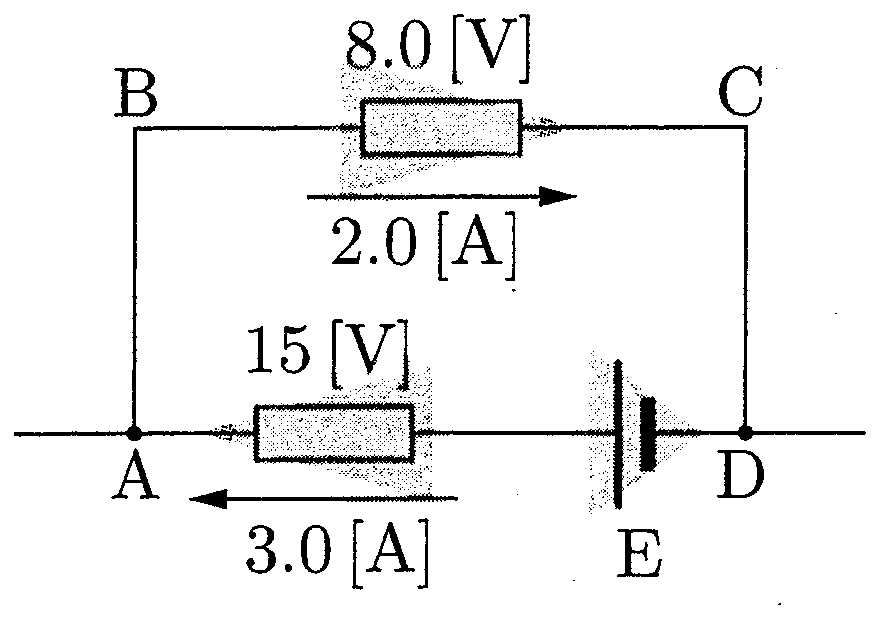
\includegraphics[keepaspectratio,width=58mm]{fig/n26_a60_zu.png}\end{center}
\ko{6} 直列接続：
       \[R=R_1+R_2=2.0+3.0=5.0\U{\Omega}\Ans\]
       並列接続：
       \[\frac{1}{R}=\frac{1}{R_1}+\frac{1}{R_2}=\frac{1}{2.0}+\frac{1}{3.0}\]
       より，
       \[R=1.2\U{\Omega}\Ans\]
\ko{7} 検流計を流れる電流が$0$なので，ブリッジの平衡条件より，
       \[2.0:R=8.0:12\]
       が成立する．よって，
       \[R=3.0\U{\Omega}\Ans\]
\end{komon}

\Rank{B問題}
\MonN{61}{電流と電荷の移動の関係}\par\nopagebreak
\begin{sisin}
$I=en\overline{v}S$を利用して，電子の平均移動速度$\overline{v}$を求めればよい．単位を$\U{m}$，$\U{kg}$，$\U{s}$，$\U{A}$の単位系に直してから代入するという点にだけ注意しよう．
\end{sisin}
\KaiHead
流れる電流の強さ$I$と自由電子密度$n$，電子の電荷の絶対値$e$，電子の平均移動速度$\overline{v}$，断面積$S$の間には
\[I=en\overline{v}S\]
の関係が成立する．問題文中で与えられた値を代入すると，
\[2.0=(1.6\times 10^{-19})\cdot(8.5\times 10^{28})\cdot\overline{v}\cdot(1.0\times 10^{-6})\]
となるのでこれを解いて，
\[\overline{v}=1.47\times 10^{-4}\fallingdotseq 1.5\times 10^{-4}\U{m/s}\Ans\]
\begin{chuu}
電子は実際には導線中で多数回衝突しながら移動しており，結果として平均して$\overline{v}\fallingdotseq 1.5\times 10^{-4}\U{m/s}$の速さで移動していくが，電子そのものが導線中で動き回る速さはこの$\overline{v}$ではない．
\end{chuu}

\MonN[\Sitei]{62}{オームの法則}\par\nopagebreak
\begin{sisin}
抵抗率$\rho$の定義式$R=\rho\dfrac{l}{S}\U{\Omega}$を利用して考える．A問題の指針でも述べたが，分母・分子を逆にしないように注意しよう．
\end{sisin}
\KaiHead
この抵抗の抵抗率を$\rho\U{\Omega\cdot m}$とすると，最初のときの抵抗値は
\[R_0=\rho\frac{l_0}{S_0}\U{\Omega}\]
であり，これに電池をつないで電流を流したときは，オームの法則より
\[V_0=R_0I_0\]
が成立する．(1)〜(3)の各設問のときに流れる電流の強さを$I_1\sim I_3\U{A}$とする．
\begin{komon}
\ko{1} このとき，オームの法則より，
       \[kV_0=R_0I_1\]
       であるから，
       \[I_1=kI_0\U{A}\Ans\]
\ko{2} このときの抵抗値は，
       \[R_2=\rho\frac{kl_0}{S_0}=kR_0\U{\Omega}\]
       であり，オームの法則より，$V_0=R_2I_2$であるから，
       \[I_2=\frac{1}{k}I_0\U{A}\Ans\]
\ko{3} このときの抵抗値は，
       \[R_3=\rho\frac{l_0}{kS_0}=\frac{1}{k}R_0\U{\Omega}\]
       であり，オームの法則より，$V_0=R_3I_3$であるから，
       \[I_3=kI_0\U{A}\Ans\]
\end{komon}
\begin{bekkai}
次のように考えてしまうと，ほとんど数式なしで答えが直観的に分かる．

オームの法則より$I=\dfrac{V}{R}$であるから，流れる電流の強さは起電力の大きさに比例し，抵抗値に反比例する．また，抵抗率の定義式$R=\rho\dfrac{l}{S}$より，抵抗値は抵抗の長さに比例し，抵抗の断面積に反比例する．よって，
\begin{komon}
\ko{1} 起電力を$k$倍にすれば流れる電流は$k$倍になる．
\ko{2} 抵抗の長さを$k$倍にすれば抵抗値が$k$倍になるので，流れる電流は$\dfrac{1}{k}$倍になる．
\ko{3} 抵抗の断面積を$k$倍にすれば抵抗値が$\dfrac{1}{k}$倍になるので，流れる電流は$k$倍になる．
\end{komon}
\end{bekkai}

\MonN[\Sitei]{63}{電気抵抗の加速モデル}\par\nopagebreak
\begin{sisin}
電気抵抗が生じる原因を推測する問題として有名なのは，例題12で扱った抵抗力モデルと，本問で扱う加速モデルの二つである．本問は誘導付きの穴埋め形式なので比較的容易に解くことができると思われるが，考え方をよく理解しておいて欲しい．
\end{sisin}
\KaiHead
\begin{komon}
\ko{1} 長さ$l\U{m}$の区間に電位差$V\U{V}$が生じているので，電場の強さは
       \[E=\frac{V}{l}\U{V/m}\Ans\]
       であり，電場の向きは高電位側から低電位側向き，すなわち$\mathrm{A}\to\mathrm{B}$向きである．
\ko{2} 電子は負電荷であるから，電場の向きとは逆向き，すなわち左向きに大きさ$eE\U{N}$の力を受ける．よって電子の運動方程式は，$ma=eE$．これに(1)を代入すれば，
       \[ma=e\frac{V}{l}\Ans\]
\ko{3} これを解いて，
       \[a=\frac{eV}{ml}\U{m/s^2}\Ans\]
\ko{4} 加速度$a$の等加速度直線運動であるから，電子の持つ衝突直前の速さは，
       \[v_{\max}=0+a\cdot T=\frac{eTV}{ml}\U{m/s}\Ans\]
\ko{5} 図(d)より，電子の平均移動速度は最大の速さの半分である．よって，
       \[\overline{v}=\frac{1}{2}v_{\max}=\frac{eTV}{2ml}\U{m/s}\Ans\]
\ko{6} 電流の定義より，流れる電流の強さは
       \[I=en\overline{v}S=\frac{ne^2TS}{2ml}V\U{A}\Ans\]
\ko{7} オームの法則$V=RI$の式と(6)を比較することにより，この金属棒の抵抗値は，
       \[R=\frac{2ml}{ne^2TS}\U{\Omega}\Ans\]
\ko{8} (7)式から定数部分を分離すると，
       \[R=\frac{2m}{ne^2T}\cdot\frac{l}{S}\U{\Omega}\]
       ゆえ，断面積の1乗に反比例する．\Ans
\ko{9} (8)より，長さの1乗に比例する．\Ans
\ko{10} 衝突直前に持っていた運動エネルギー$\dfrac{1}{2}mv_{\max}^2\U{J}$がすべて失われるのだから，
       \[\frac{1}{2}mv_{\max}^2=\frac{e^2T^2V^2}{2ml^2}\U{J}\Ans\]
\ko{11} 金属棒の体積は$Sl\U{m^3}$であるから電子の総数は，
       \[N=nSl\ \text{個}\Ans\]
\ko{12} 電子は時間間隔$T\U{s}$で衝突するので，1秒間あたりの衝突回数は，
       \[\frac{1}{T}\ \text{回}\Ans\]
\ko{13} 一つの電子が一回の衝突で与えるエネルギーが(10)であることに注意すると，
       \[\begin{aligned}
         &\frac{e^2T^2V^2}{2ml^2}\times(nSl)\times\frac{1}{T}\\
         &=\frac{ne^2ST}{2ml}V^2\U{W}\Ans
       \end{aligned}\]
\ko{14} $I=\dfrac{ne^2TS}{2ml}V\U{A}$であるから，(13)を整理すると，
       \[\frac{ne^2ST}{2ml}V^2=\Bigl(\frac{ne^2TS}{2ml}V\Bigr)\cdot V=IV\U{W}\Ans\]
\end{komon}
\begin{bsHosoku}{参考}
{\gtfamily モデルについて}

なぜ電気抵抗が生じるのかについては現在でこそ詳しく知られているが，かつては電子などの微粒子の運動は詳しくは知られておらず，なぜ電気抵抗が生じるのか，またなぜオームの法則$V=RI$が成立するのかが分からなかった．そこで，先人たちは，「おそらく抵抗の中ではこんなことが起きているのだろう」ということを推定し（これをモデルという），そのモデルを運動方程式などを用いて解くことを行った．もちろんこのモデルというのは半ば「当てずっぽう」として考え出したものであるから本当に正しいとは限らないが，もし運動方程式を解いて出てきた答えが，例えば$V=RI$の関係式を満たしているのであれば，もしかしたらそのモデルが抵抗の中で実際に起こっている現象そのものなのかもしれないわけである．つまり，現実に観測される現象のうち，もし一つでもそのモデルによって説明できないものがあるのであれば，そのモデルは現実とは異なると言える．また逆に，観測されるすべての現象がそのモデルによって完璧にすべて説明されるのであれば，そのモデルは現実に抵抗内で起こっていることそのものであると考えることができる．残念ながら，例題12と本問で扱った二つのモデルは，すべての現象については説明できないことが知られているが，この二つのモデルは比較的簡単であり，またオームの法則$V=RI$や抵抗率の式$R=\rho\dfrac{l}{S}$については説明がうまくつくため，高校向けの物理としてよく引き合いに出されている．実際の抵抗内で本当に起こっていることはもっと非常に複雑な事象である．
\end{bsHosoku}

\MonN{64}{抵抗の温度変化}\par\nopagebreak
\begin{sisin}
抵抗値・抵抗率の温度依存性を示す関係式$R=R_0(1+\alpha t)\U{\Omega}$および$\rho=\rho_0(1+\alpha t)\U{\Omega\cdot m}$を覚えておけば(1)は簡単な問題である．ただし，温度については$\U{^\circ C}$単位を利用している点に注意すること．

(2)の判定方法を覚えておくこと．$I=\dfrac{1}{R}V$の式において，本来，理想的なオーム抵抗の場合には抵抗値$R$の値が温度によって変化しないため，原点を通る直線となる．問題で与えられたグラフは，電圧を増加させていったとき理想的なオーム抵抗で期待される直線よりも下側に来ているので，電流が次第に流れにくくなっていくことが読み取れる．
\end{sisin}
\KaiHead
\begin{komon}
\ko{1} 温度$t\U{^\circ C}$におけるこの物質の抵抗値を$R\U{\Omega}$とする．抵抗値の温度係数は抵抗率の温度係数と同じであるから，$R=R_0(1+\alpha t)$が成立する．温度が$t_1$，$t_2\U{^\circ C}$のときについての抵抗値の式を立てると，
       \[R_1=R_0(1+\alpha t_1),\qquad R_2=R_0(1+\alpha t_2)\]
       であるから，この2式を連立することにより，
       \[\left\{\begin{aligned}
         R_0&=\frac{R_1t_2-R_2t_1}{t_2-t_1}\U{\Omega}\\
         \alpha&=\frac{R_2-R_1}{R_1t_2-R_2t_1}\U{/K}
       \end{aligned}\right.\Ans\]
\ko{2} 理想的なオーム抵抗であれば，温度によらず抵抗値が不変であるから，電流-電圧曲線は$I=\dfrac{1}{R}V$の式に従って直線になるはずである（次図の点線）．
       \begin{center}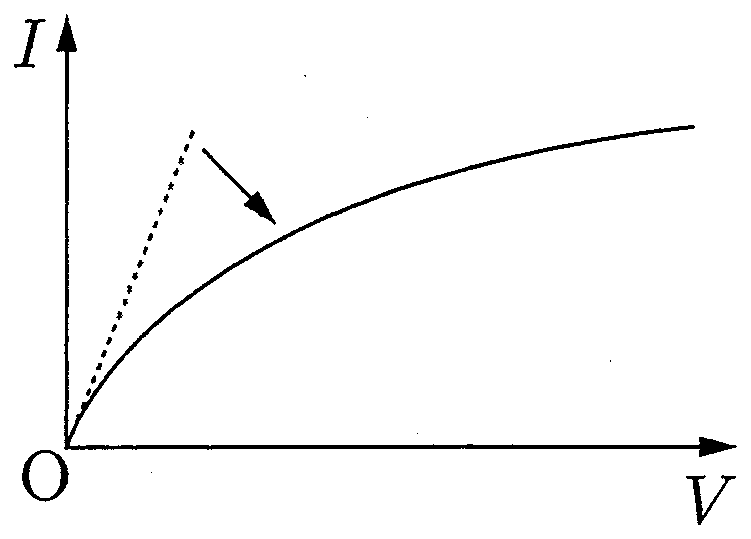
\includegraphics[keepaspectratio,width=44mm]{fig/n26_a64_zu.png}\end{center}
       しかし実際には，電圧をかけてもそれより少ない電流しか流れていないので，この物質は電圧を高くするにつれて抵抗値が増加していくと考えられる．

       また，一般にかける電圧を増加させる（それと同時に流れる電流も増加する）と，発生するジュール熱が増加するので，電圧・電流が大きいほど発熱量が大きく，物質の温度は高くなると考えられる．

       以上より，この物質は，温度が高くなると抵抗値が大きくなるという性質を持つことが分かる．よって温度係数は{\gtfamily 正}である．\Ans

       また，金属は温度係数が正，半導体は温度係数が負となるので，この物質は{\gtfamily \MARU{1}の金属}であると考えられる．\Ans
\end{komon}
\begin{bsHosoku}{参考}
金属では温度が高くなると陽イオンの運動が激しくなり，電子と陽イオンの衝突確率が高くなるので抵抗値が大きくなる．よって温度係数が正となる．

また半導体（14族のシリコン・ゲルマニウムに13族・15族の元素を極微量混ぜたもの）では温度が高くなると共有結合の一部が切断し，電気伝導に寄与できる電子の数が増加するので電流が流れやすくなる．すなわち抵抗値が小さくなるので，温度係数は負となる．
\end{bsHosoku}

\MonN{65}{電流計・電圧計}\par\nopagebreak
\begin{sisin}
例えば問題の図(a)のように電流計，電圧計を挿入すると，電圧計にも（非常に微小ではあるが）電流が流れ込んでしまうため，抵抗の両端間の電位差は正しく測定できるが，抵抗を流れる電流は精密には測定できない．そこで，異なる2パターンの電流計・電圧計の挿入の仕方をし，回路のキルヒホッフの第二法則を用いて抵抗の抵抗値を求めよう，というのが本問の趣旨である．問題を解く上では，電流計・電圧計をそれぞれ抵抗値$r_{\mathrm{A}}\U{\Omega}$，$r_{\mathrm{V}}\U{\Omega}$の抵抗であると考えてキルヒホッフの第二法則を適用して立式していけばよい．
\end{sisin}
\KaiHead
電圧計・電流計を内部抵抗部分とメーター部分に分け，さらに問題文で与えられた測定値を元に考えると，次のようになる．
\begin{center}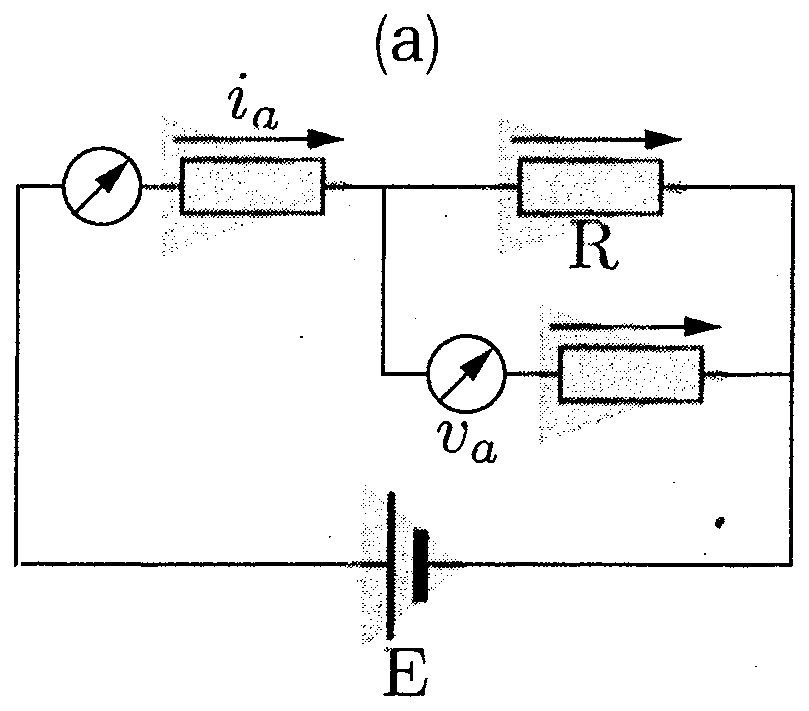
\includegraphics[keepaspectratio,width=52mm]{fig/n26_a65_a.png}\\[2mm]
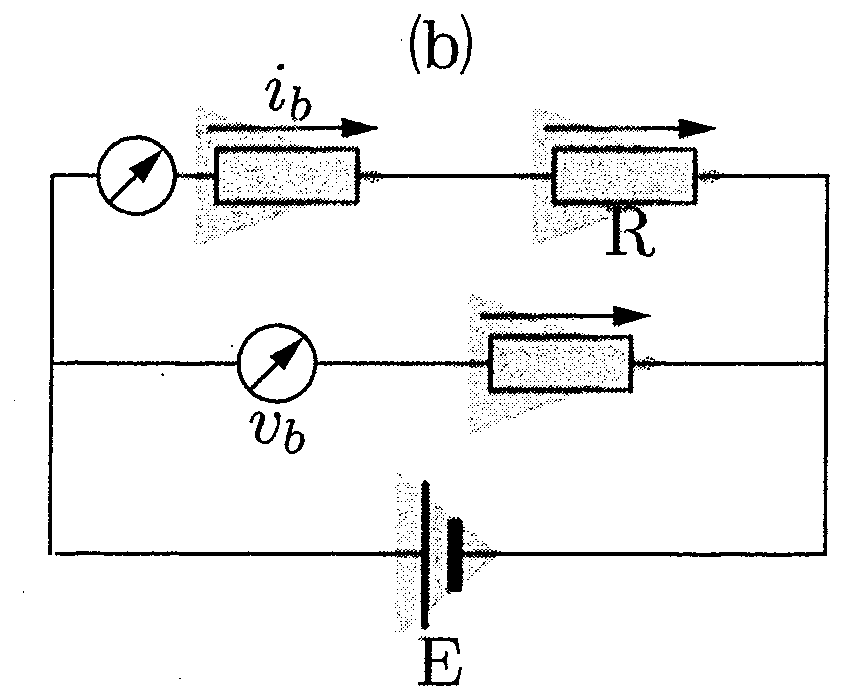
\includegraphics[keepaspectratio,width=52mm]{fig/n26_a65_b.png}\end{center}
メーター部分には抵抗がないので電圧がかからないことに注意すると，まず(b)の測定より，電圧計は電池に直接並列につながっているので，この電池の起電力は，
\[E=v_b=6.00\U{V}\Ans\]
次に，図(a)の下側ループ（電池－電流計－電圧計のループ）に対してキルヒホッフの第二法則より，
\[E=r_{\mathrm{A}}i_a+v_a\]
であるからこれを解いて，電流計の内部抵抗は
\[r_{\mathrm{A}}=\frac{6.00-4.92}{0.540}=2.00\U{\Omega}\Ans\]
これを元に，図(b)の外周ループに対してキルヒホッフの第二法則を用いると，
\[E=r_{\mathrm{A}}i_b+Ri_b\]
これを解いて，抵抗の抵抗値は
\[R=\frac{6.00}{0.500}-2.00=10.0\U{\Omega}\Ans\]
以上を元に，図(a)の右上ループに着目すると，抵抗には$v_a=4.92\U{V}$の電圧がかかっているので，
\[I=\frac{v_a}{R}=0.492\U{A}\]
の電流が流れている．よって，図(a)において電圧計に流れ込む電流は
\[i_a-I=0.048\U{A}\]
であるから，電圧計の内部抵抗値は，
\[r_{\mathrm{V}}=\frac{v_a}{0.048}\fallingdotseq 1.0\times 10^2\U{\Omega}\Ans\]
% 原本は「≒103[Ω]」．4.92/0.048＝102.5 で，0.048 が有効数字2桁なので 1.0×10^2 とした．
\begin{chuu}
先に回路内のループにキルヒホッフの第二法則をすべて用いてから解くのも一つの方法であるが，本問の場合は未知数が非常に多いためどこから攻めていけばよいのかが分かりにくくなる．そこで上述した解答のように，分かる部分から順番に，適宜キルヒホッフの第二法則を用いて考えていった方が容易に問題を解くことができる．
\end{chuu}

\Rank{C問題}
\MonN{66}{すべり抵抗}\par\nopagebreak
\begin{sisin}
抵抗値は長さに比例するので，$\mathrm{AC}$間，$\mathrm{CB}$間それぞれの抵抗値は$R_0\U{\Omega}$を長さで分配した値となる．$\mathrm{AC}$間，$\mathrm{CB}$間をそれぞれ抵抗に置き換え，さらに電流の流れを元にキルヒホッフの第二法則を立てよう．
\end{sisin}
\KaiHead
\begin{komon}
\ko{1} 抵抗値は長さに比例するので，$\mathrm{AC}$，$\mathrm{CB}$の抵抗値をそれぞれ$R_1$，$R_2\U{\Omega}$とすると，
       \[R_1=\frac{x}{l}R_0,\qquad R_2=\frac{l-x}{l}R_0\]
       である．また題意を元に電流の流れを記入し，それを元に各抵抗にかかる電圧を図示すると次図のようになる．
       \begin{center}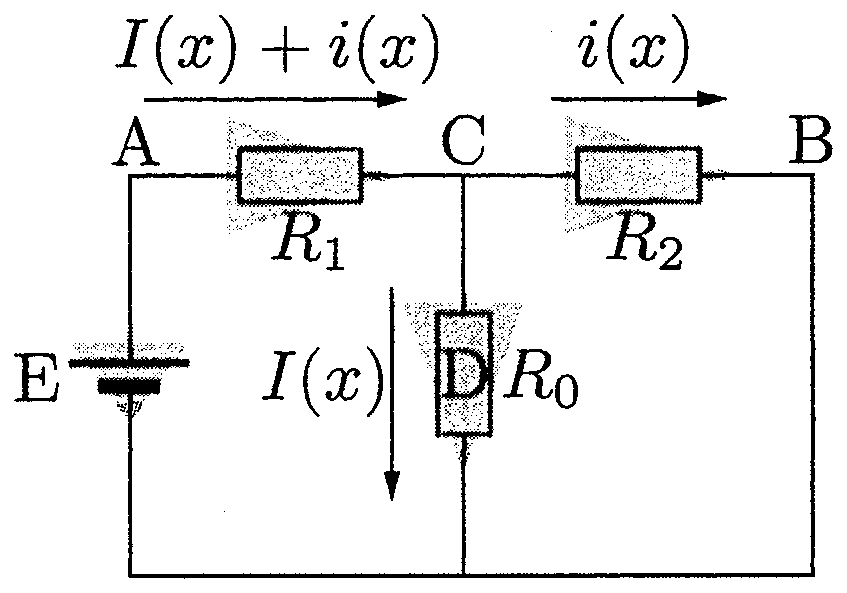
\includegraphics[keepaspectratio,width=56mm]{fig/n26_a66_zu.png}\end{center}
       よってこの回路にキルヒホッフの第二法則を用いると，
       % 原本は第1式の左辺が「W=」になっていた（誤植．直後の代入後の式では E）．
       \[\begin{aligned}
         E&=R_1\{I(x)+i(x)\}+R_0I(x)\\
         0&=R_0I(x)-R_2i(x)
       \end{aligned}\]
       これらに$R_1$，$R_2$を代入して，
       \[\left\{\begin{aligned}
         E&=\frac{x}{l}R_0\{I(x)+i(x)\}+R_0I(x)\\
         0&=R_0I(x)-\frac{l-x}{l}R_0i(x)
       \end{aligned}\right.\Ans\]
\ko{2} 以上2式より$I(x)$を消去して$i(x)$を求めると，
       \[i(x)=\frac{l^2}{l^2+lx-x^2}\cdot\frac{E}{R_0}\U{A}\Ans\]
       ここで分母に着目すると，
       \[l^2+lx-x^2=\frac{5}{4}l^2-\Bigl(x-\frac{l}{2}\Bigr)^2\]
       であり，$0\leqq x\leqq l$であることから$x=\dfrac{l}{2}$のとき，分母最大となる．よって，$i(x)$が最小となるのは，
       \[x=x_0=\frac{l}{2}\U{m}\Ans\]
       のときである．
\end{komon}

\MonN{67}{電池の内部抵抗}\par\nopagebreak
\begin{sisin}
内部抵抗は一般には非常に小さいため無視してよいことが多いが，無視できない場合には電池を内部抵抗と起電力分の電圧をもつ電池とに分けて（直列に接続して）描き直して考える（26.7）．本問のタイプの問題ではその最大値を求める際に相加平均と相乗平均の関係を利用するとあっさりとカタがつくので，この式の形を見たら相加平均と相乗平均の関係を利用する，ということを覚えておくこと．
\end{sisin}
\KaiHead
\begin{komon}
\ko{1} 電池を内部抵抗と起電力分の電圧をもつ電池とに分けて回路の図を描き直すと，次図の通りとなる．
       \begin{center}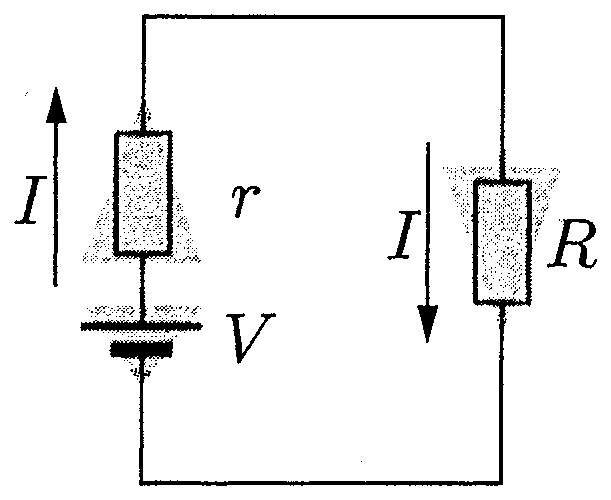
\includegraphics[keepaspectratio,width=40mm]{fig/n26_a67_zu.png}\end{center}
       この回路についてキルヒホッフの第二法則より立式すると，$V=rI+RI$．ゆえ，
       \[I=\frac{V}{R+r}\U{A}\Ans\]
\ko{2} 抵抗で消費する電力$P$は，この抵抗の抵抗値$R$および電流値$I$を用いて，$P=RI^2$であるから，(1)を代入して，
       \[P=R\Bigl(\frac{V}{R+r}\Bigr)^2=\frac{R}{(R+r)^2}V^2\U{W}\Ans\]
       ここで，式の分母分子を$(\sqrt{R})^2$で割り算すると，
       \[P=\frac{V^2}{\Bigl(\sqrt{R}+\dfrac{r}{\sqrt{R}}\Bigr)^2}\]
       となるが，分母の括弧内に対して相加平均と相乗平均の関係を利用すると，
       \[\sqrt{R}+\frac{r}{\sqrt{R}}\geqq 2\sqrt{\sqrt{R}\cdot\frac{r}{\sqrt{R}}}=2\sqrt{r}\]
       である．$P\U{W}$が最大となるのは分母が最小となるときであるから，相加平均と相乗平均の関係の等号が成立するとき，すなわち
       \[\sqrt{R}=\frac{r}{\sqrt{R}}\iff R=r\U{\Omega}\Ans\]
       となるとき，外部抵抗で消費する電力が最大となる．
\end{komon}
\begin{bekkai}
まともに数学的に処理するには，$P\U{W}$の式を$R$の関数とみなして処理する．
\[\frac{d}{dR}\Bigl\{\frac{R}{(R+r)^2}\Bigr\}=-\frac{R-r}{(R+r)^3}\]
であるから，これの正負を考えて$P$の$R$に対する増減を考えることにより，$P$は$R=r$のとき最大値$\dfrac{V^2}{4r}\U{W}$をとることが分かる．
% 原本は最大値を V^2/(4R) と書いていた．R=r を代入した値なので同じだが，r で書くべき．

また(2)より，『外部抵抗における消費電力を最大にするためには，外部抵抗の値を電池の内部抵抗の値に等しくすればよい』ことがわかる．この事実は頭の片隅に置いておくとよい．
\end{bekkai}

\MonN{68}{合成抵抗}\par\nopagebreak
\begin{sisin}
与えられた図のままでは非常に考えにくいので，回路がどのように対称になっているのかを明らかにするように回路図を書き換えた上で考えよう．本問の場合は$\mathrm{a}$，$\mathrm{c}$間に電池を接続するのだから，真上から見ると回路の対称性が明らかになる．(1)の証明方法については対称回路の電流分布を決める際の一つのテクニックなので，覚えておくとよい（26.9）．
\end{sisin}
\KaiHead
\begin{komon}
\ko{1} 回路を真上から見ると次図のようにみなせる．
       \begin{center}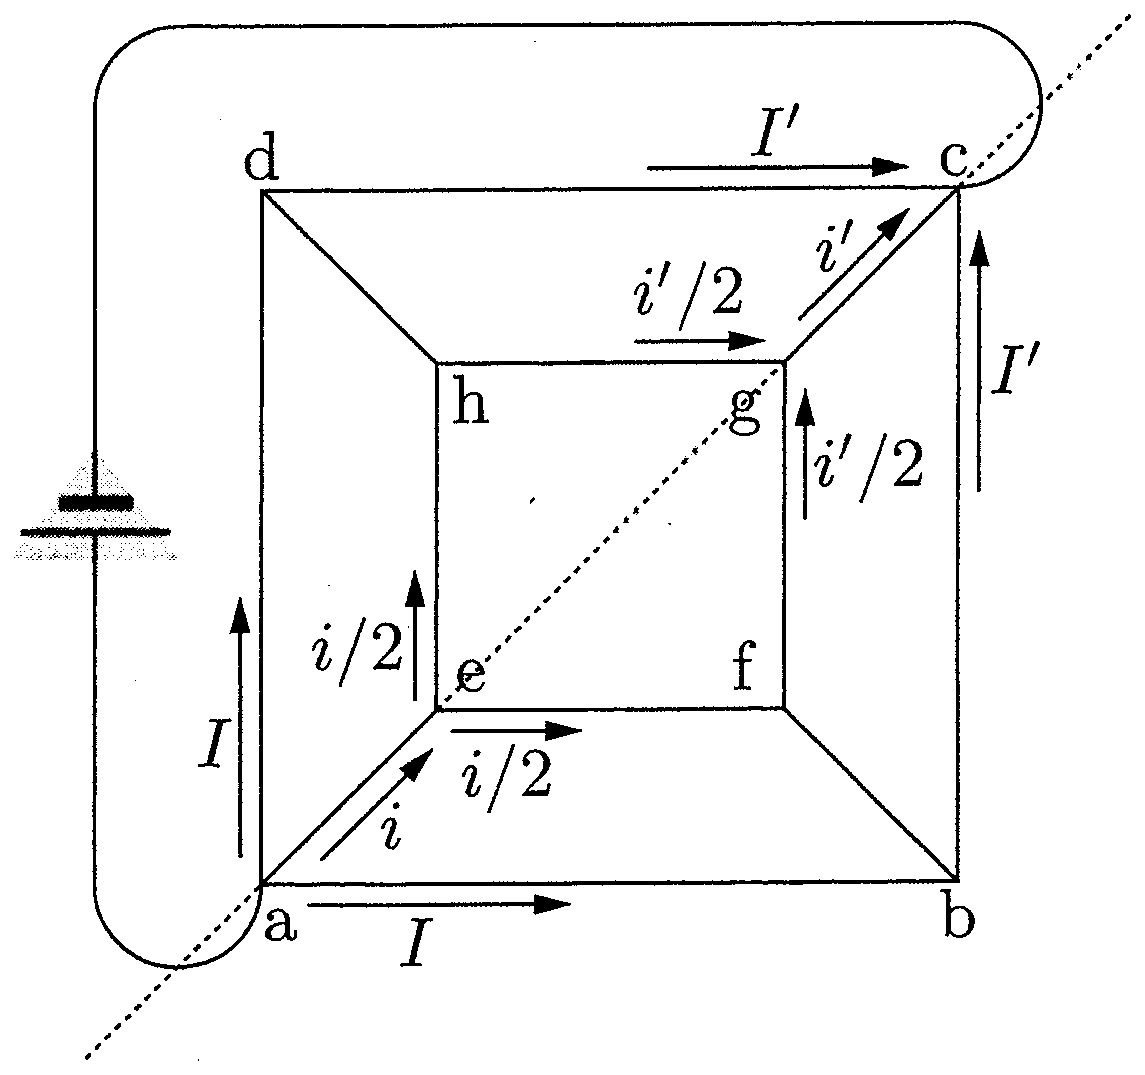
\includegraphics[keepaspectratio,width=56mm]{fig/n26_a68_zu1.png}\end{center}
       $\mathrm{ac}$間に図のように電池をつないだときに流れる電流について考える．このとき，回路は$\mathrm{ac}$を結ぶ直線に対して対称であるから，$\mathrm{a}$点から$\mathrm{b}$，$\mathrm{d}$点に向かう電流の強さは等しく（これを$I\U{A}$とする），また$\mathrm{e}$点から$\mathrm{h}$，$\mathrm{f}$点に向かう電流の強さも等しい（これを$\dfrac{i}{2}\U{A}$とする）．また$\mathrm{c}$点に吸い込まれる電流に着目すると，$\mathrm{b}$，$\mathrm{d}$点から$\mathrm{c}$点に向かう電流の強さは等しく（これを$I^\prime\U{A}$とする），また$\mathrm{h}$，$\mathrm{f}$点から$\mathrm{g}$点に向かう電流の強さも等しい（これを$\dfrac{i^\prime}{2}\U{A}$とする）．

       ここで，もし電池を接続する向きを逆にしたとすると，電圧降下の向きがすべて逆転するため，各抵抗に流れる電流は大きさが同じまま向きがすべて反転する．
       \begin{center}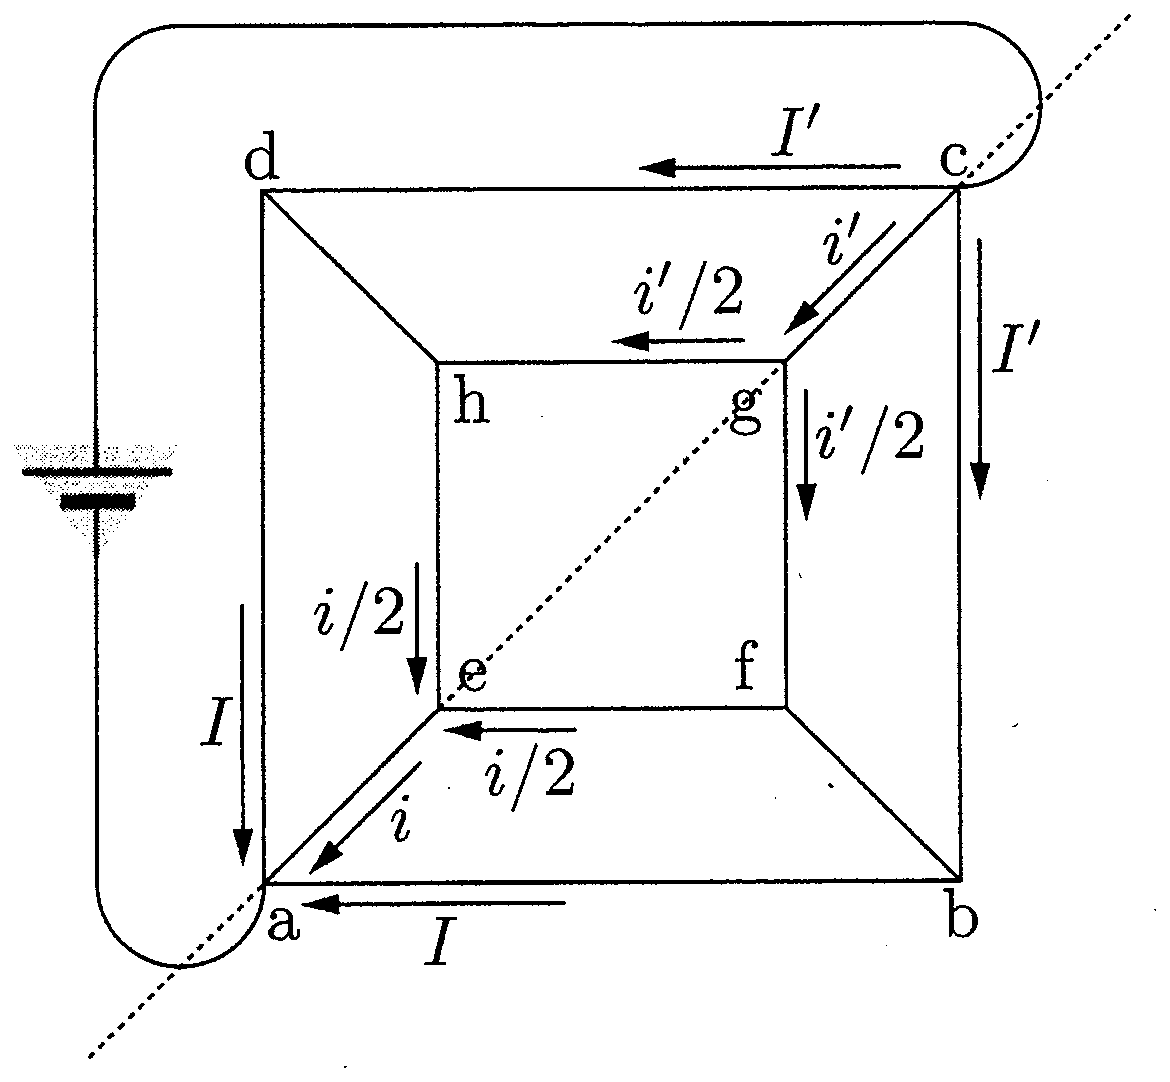
\includegraphics[keepaspectratio,width=56mm]{fig/n26_a68_zu2.png}\end{center}
       この回路図を180度回転させると最初の回路と全く同じ回路が得られ，この二つを比較すると，
       \[I=I^\prime,\qquad i=i^\prime\]
       であることが分かる．ゆえに電流分布は次図のようになっている．
       \begin{center}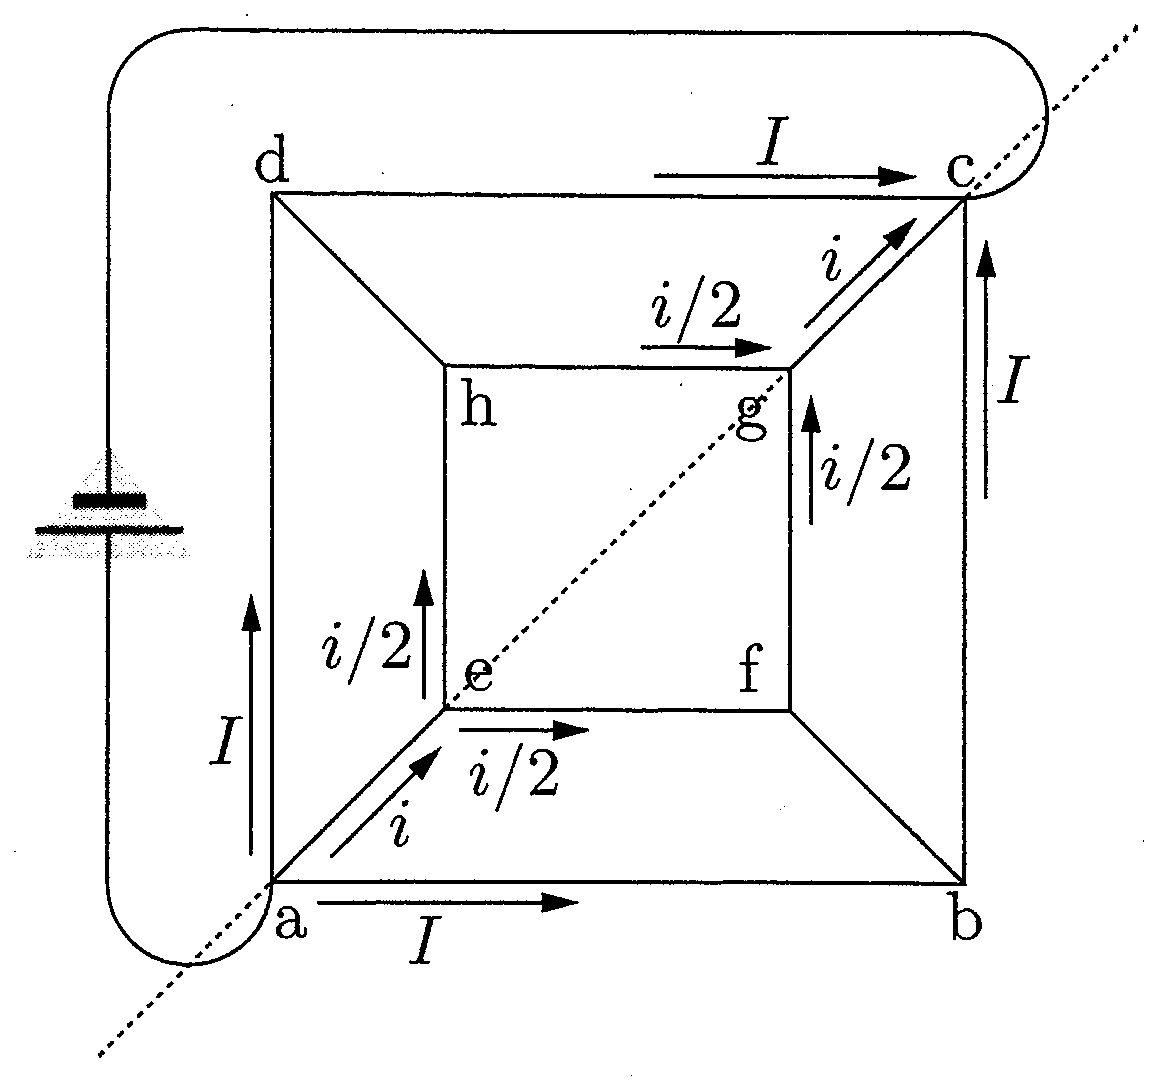
\includegraphics[keepaspectratio,width=56mm]{fig/n26_a68_zu3.png}\end{center}
       この図から分かるように，辺$\mathrm{dh}$および$\mathrm{fb}$には電流は流れない．以上より，
       \[\text{辺}\,\mathrm{dh}\ \text{および辺}\,\mathrm{fb}\Ans\]
       の二つの抵抗線を外しても電流分布に変化がないので，合成抵抗に変化はない．
\ko{2} まず底面について$\mathrm{eg}$間の合成抵抗を求めると，これは$\mathrm{ehg}$および$\mathrm{efg}$の並列接続になっているので，
       \[\Bigl(\frac{1}{2r}+\frac{1}{2r}\Bigr)^{-1}=r\U{\Omega}\]
       である．よって$\mathrm{ae}$，（$\mathrm{fh}$），$\mathrm{gc}$と通る底面側の合成抵抗値は，
       \[r+r+r=3r\U{\Omega}\]
       である．これと$\mathrm{abc}$，$\mathrm{adc}$の抵抗が並列接続されているので，全合成抵抗値は，
       \[\Bigl(\frac{1}{3r}+\frac{1}{2r}+\frac{1}{2r}\Bigr)^{-1}=\frac{3}{4}r\U{\Omega}\Ans\]
\end{komon}

\end{multicols}
